\chapter{能量、动量与电磁场}

最后一讲以一处修正开始，以将出现在爱因斯坦方程右端的那个对象结束。这条路线并非绕道。首先必须明确电场的一个符号约定；随后必须区分动量的三种不同含义。只有完成这些准备工作之后，场论才能被读作在空间每一点都有一个自由度的普通力学。于是哈密顿量、局域能量密度、诺特动量、电磁能量与坡印廷矢量便在一个连续的论证中依次出现。

\section{必须始终一致采用的约定}

预备笔记本应发给全班，但这个问题重要到足以当众讲清楚。拜伦注意到的不一致并不在课程记号内部，而在于该记号与几乎其他所有地方所用的记号之间。这是重新推导方程的一种职业风险：一个内部自洽的私人约定可能偏离公共约定。

记\(\mathbf E_M\)为标准麦克斯韦--富兰克林约定，\(\mathbf E_L\)为前几讲所用的约定。以课程的协变分量\(A_0\)表示，它们为
\begin{align}
\mathbf E_M
  &= -\dot{\mathbf A}+\boldsymbol{\nabla}A_0,
&
\mathbf E_L
  &= +\dot{\mathbf A}-\boldsymbol{\nabla}A_0
   =-\mathbf E_M .
\label{eq:two-electric-conventions}
\end{align}
许多书则引入标势\(\Phi=-A_0\)；于是第一个公式写作
\(\mathbf E_M=-\dot{\mathbf A}-\boldsymbol{\nabla}\Phi\)。
磁场不变：
\begin{equation}
\mathbf B=\boldsymbol{\nabla}\times\mathbf A.
\label{eq:B-from-A-opening}
\end{equation}

在\(c=1\)的有理化单位制中，标准麦克斯韦--富兰克林方程为
\begin{align}
\boldsymbol{\nabla}\times\mathbf E_M&=-\dot{\mathbf B},
&
\boldsymbol{\nabla}\cdot\mathbf B&=0,
\nonumber\\
\boldsymbol{\nabla}\times\mathbf B&=\dot{\mathbf E}_M+\mathbf J_F,
&
\boldsymbol{\nabla}\cdot\mathbf E_M&=\rho_F .
\label{eq:maxwell-franklin}
\end{align}
本杰明·富兰克林的历史选择确定了电荷的符号：在此约定中电子为负。课程约定还反转了源标签，
\begin{equation}
\mathbf J_L=-\mathbf J_F,
\qquad
\rho_L=-\rho_F.
\label{eq:source-convention-map}
\end{equation}
因此代入
\(\mathbf E_L=-\mathbf E_M\)便给出
\begin{align}
\boldsymbol{\nabla}\times\mathbf E_L&=+\dot{\mathbf B},
&
\boldsymbol{\nabla}\cdot\mathbf B&=0,
\nonumber\\
\boldsymbol{\nabla}\times\mathbf B&=-\dot{\mathbf E}_L-\mathbf J_L,
&
\boldsymbol{\nabla}\cdot\mathbf E_L&=\rho_L .
\label{eq:maxwell-course-convention}
\end{align}

\begin{figure}[H]
\centering
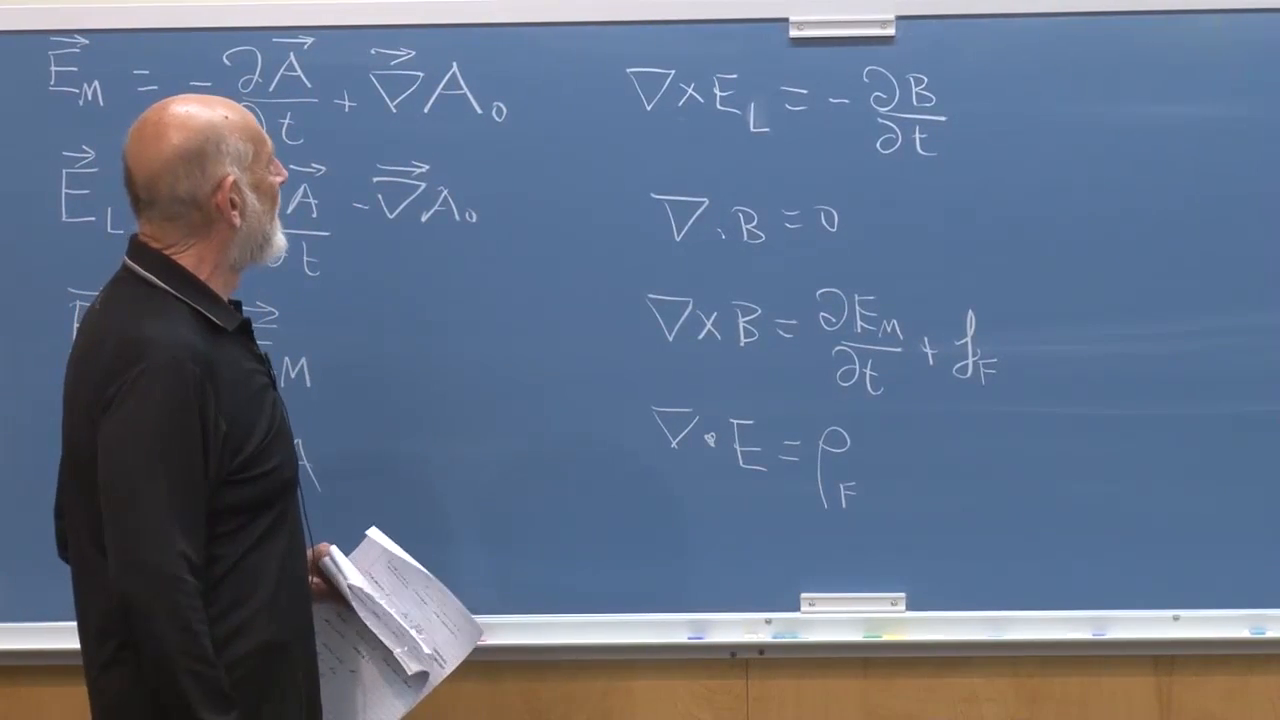
\includegraphics[width=\linewidth]{lecture_10_figure_01.png}
\caption{麦克斯韦--富兰克林约定与课程约定之间的完整板书对照。}
\par\smallskip
\textit{讲课帧：00:07:10。}
\end{figure}

没有任何可测量量依赖于选择哪本词典。要紧的是自洽性，尤其是在把计算出的场与已发表的实验值相比较时。实际的笑话在于，这类直接的数值比较在讲者自己的工作中出现得如此之少，以至于相反的符号一直未被察觉，直到全班对此提出注意。对于本章后面的电磁计算，我们将使用标准场
\(\mathbf E\equiv\mathbf E_M\)。

\section{三种被称为动量的不同量}

现在必须剖析\emph{动量}一词。机械动量、正则动量与诺特动量在简单问题中可以重合，但它们并非同一个量的三种描述。在一般系统中，它们可以有不同的数值。

\subsection{机械动量}

对于总质量为\(M\)的物体，机械动量为
\begin{equation}
\mathbf P_{\mathrm{mech}}=M\dot{\mathbf X}_{\mathrm{cm}}.
\label{eq:mechanical-momentum}
\end{equation}
对于单个粒子，\(\mathbf X_{\mathrm{cm}}\)就是它的位置。
对于复合物体，质心这一限定至关重要。

\begin{figure}[H]
\centering
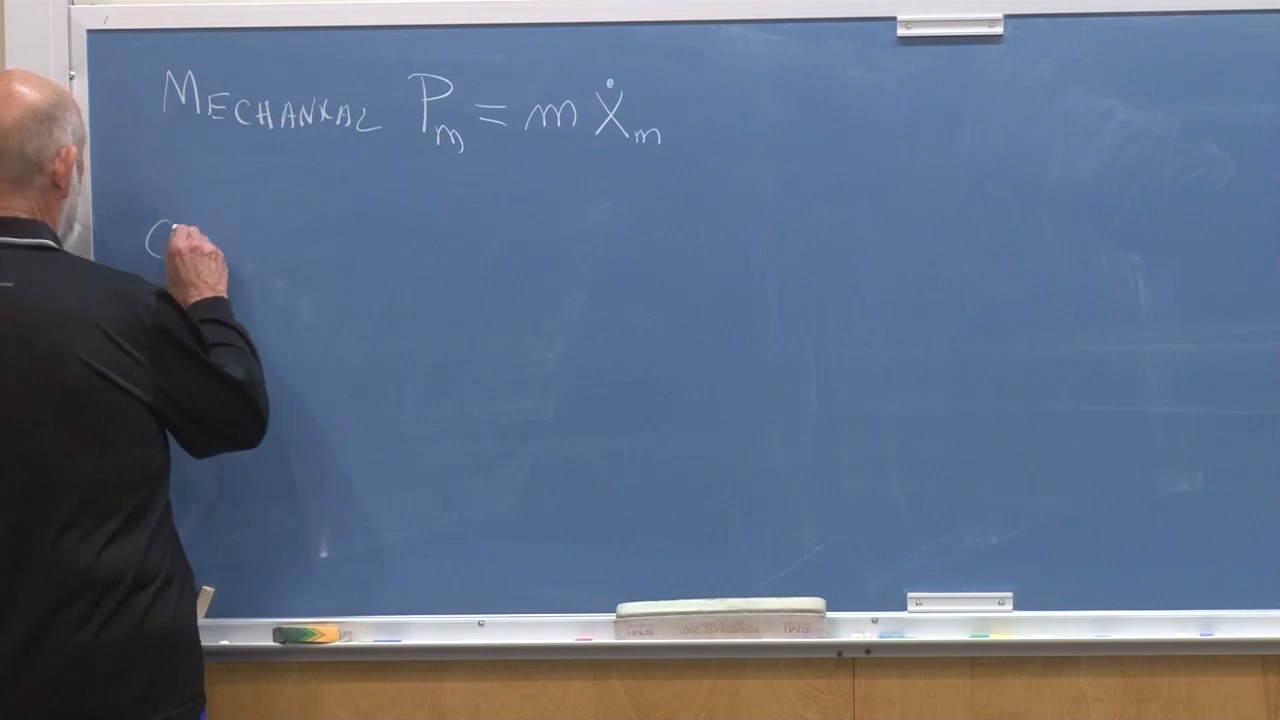
\includegraphics[width=\linewidth]{lecture_10_figure_02.png}
\caption{作为质量乘以质心速度而引入的机械动量。}
\par\smallskip
\textit{讲课帧：00:11:15。}
\end{figure}

\subsection{正则动量}

假设力学由
\(L(q_i,\dot q_i)\)描述。与\(q_i\)共轭的正则动量为
\begin{equation}
p_i=\frac{\partial L}{\partial\dot q_i}.
\label{eq:canonical-momentum}
\end{equation}
对于
\begin{equation}
L=\frac12 m\dot{\mathbf x}^{\,2}-V(\mathbf x),
\label{eq:simple-particle-lagrangian}
\end{equation}
这给出\(\mathbf p=m\dot{\mathbf x}\)，因此正则动量与机械动量恰好一致。

\begin{figure}[H]
\centering
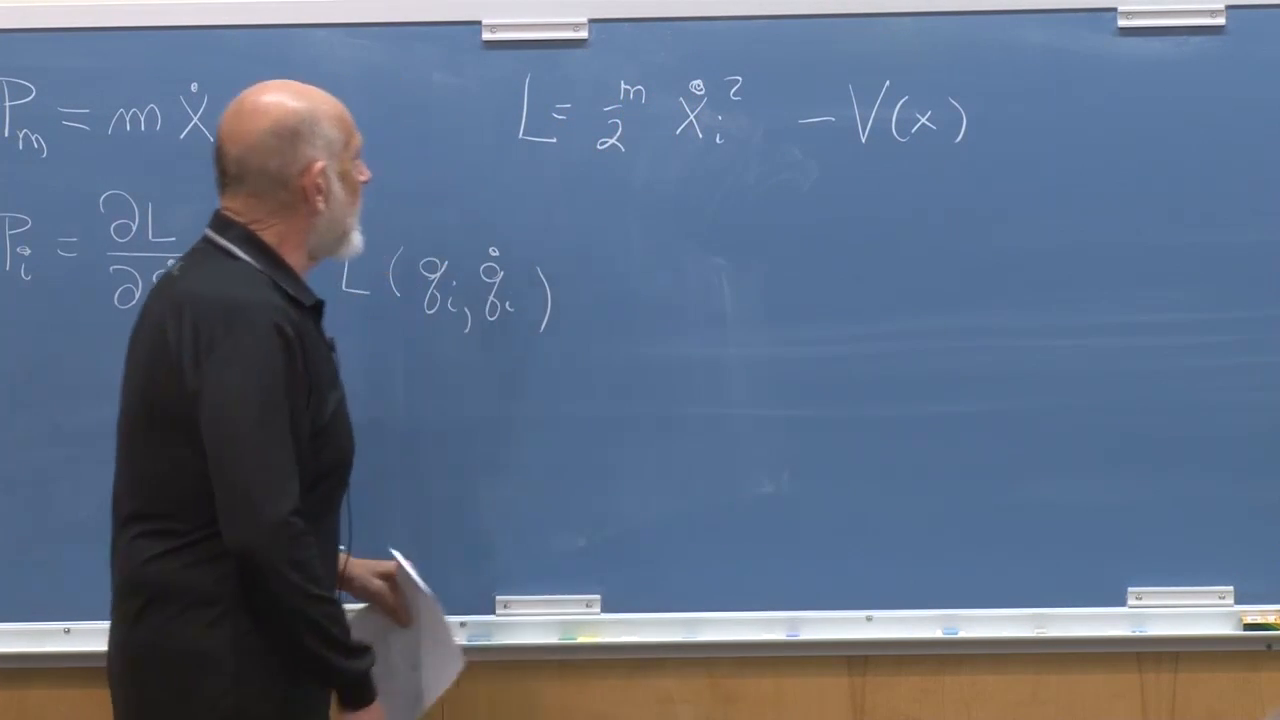
\includegraphics[width=\linewidth]{lecture_10_figure_03.png}
\caption{机械动量与正则动量并排展示在简单粒子拉格朗日量旁。}
\par\smallskip
\textit{讲课帧：00:13:40。}
\end{figure}

磁场中的带电粒子是有用的反例。以黑板上写下的符号约定，
\begin{equation}
L=\frac12m\dot{\mathbf x}^{\,2}-V(\mathbf x)
  -e\,\dot{\mathbf x}\cdot\mathbf A(\mathbf x),
\label{eq:magnetic-particle-lagrangian}
\end{equation}
因此
\begin{equation}
p_i=m\dot x_i-eA_i.
\label{eq:magnetic-canonical-shift}
\end{equation}
改变电荷或相互作用项的约定会改变所显示的符号，但不会改变这一教训：正则动量包含一个矢势贡献，并不仅仅是\(m\dot x_i\)。
哈密顿方程使用正则变量。人们之后可以把依赖于场的项移到方程的另一边，从而恢复出看似牛顿形式的加速度，但这种重新排列并不改变定义。

\begin{figure}[H]
\centering
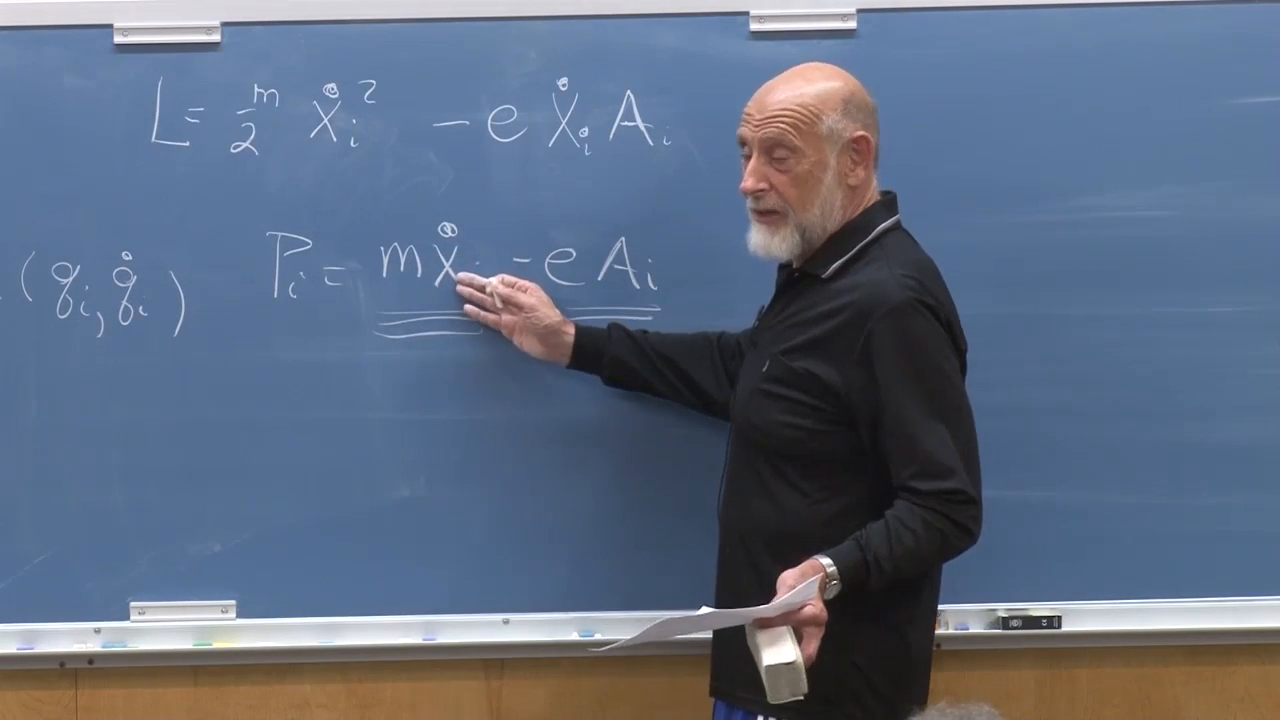
\includegraphics[width=\linewidth]{lecture_10_figure_04.png}
\caption{矢势项使正则动量偏离机械动量。}
\par\smallskip
\textit{讲课帧：00:15:50。}
\end{figure}

\subsection{诺特动量}

第三个动量是与空间平移不变性相关联的守恒荷。对于使拉格朗日量保持不变的一个无穷小对称性
\begin{equation}
q_i\longrightarrow q_i+\delta q_i
\end{equation}
诺伊特定理给出，在无穷小参数归一化意义下，
\begin{equation}
Q=\sum_i p_i\,\delta q_i.
\label{eq:noether-charge-mechanics}
\end{equation}
这里出现的\(p_i\)是正则动量。如果该对称性是均匀平移，并且正则动量恰好等于机械动量，则\(Q\)就化为熟悉的总动量。在较不简单的系统中，这种巧合必须被证明，而不能被假定。

\begin{figure}[H]
\centering
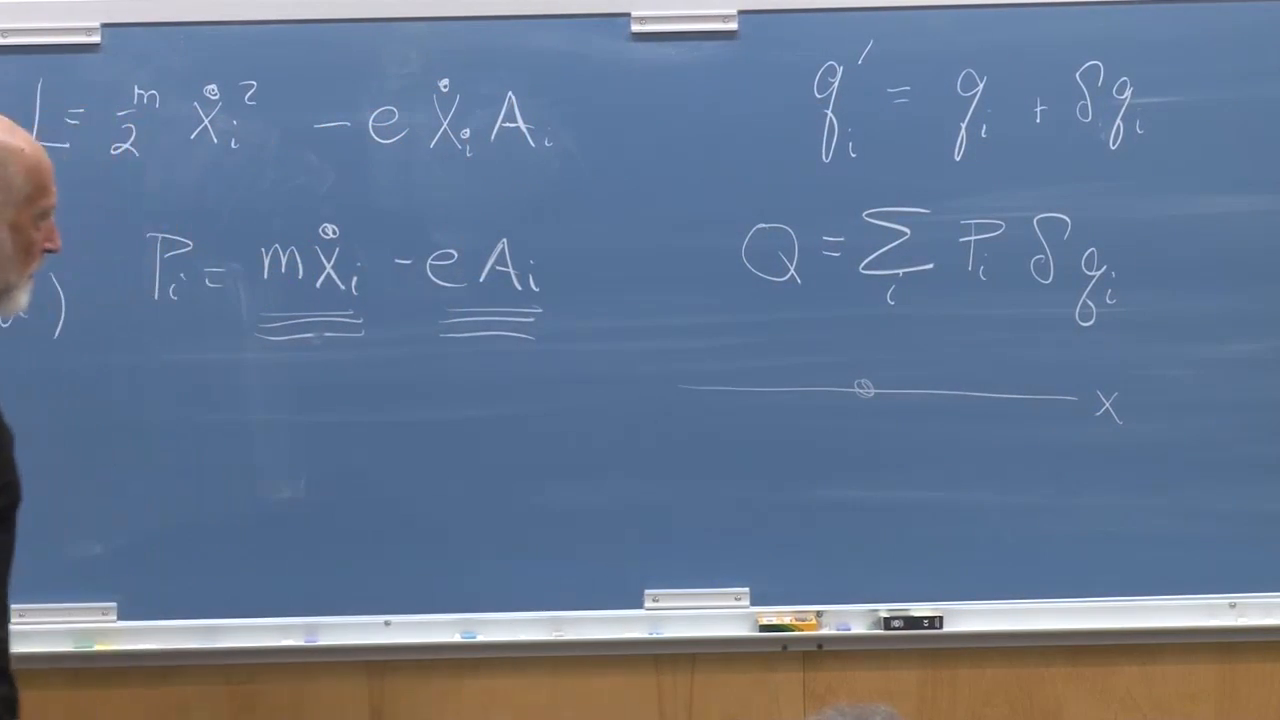
\includegraphics[width=\linewidth]{lecture_10_figure_05.png}
\caption{由正则动量和坐标的无穷小变化组装而成的诺伊特荷。}
\par\smallskip
\textit{授课画面：00:19:00。}
\end{figure}

\section{作为哈密顿量的能量}

空间平移导致动量；时间平移导致能量。如果拉格朗日量没有显式的时间依赖，则哈密顿量
\begin{equation}
H=\sum_i p_i\dot q_i-L
\label{eq:hamiltonian-definition}
\end{equation}
是守恒的。这是拉格朗日量的勒让德变换，而不是一条通过观察来改变符号的规则。

\begin{figure}[H]
\centering
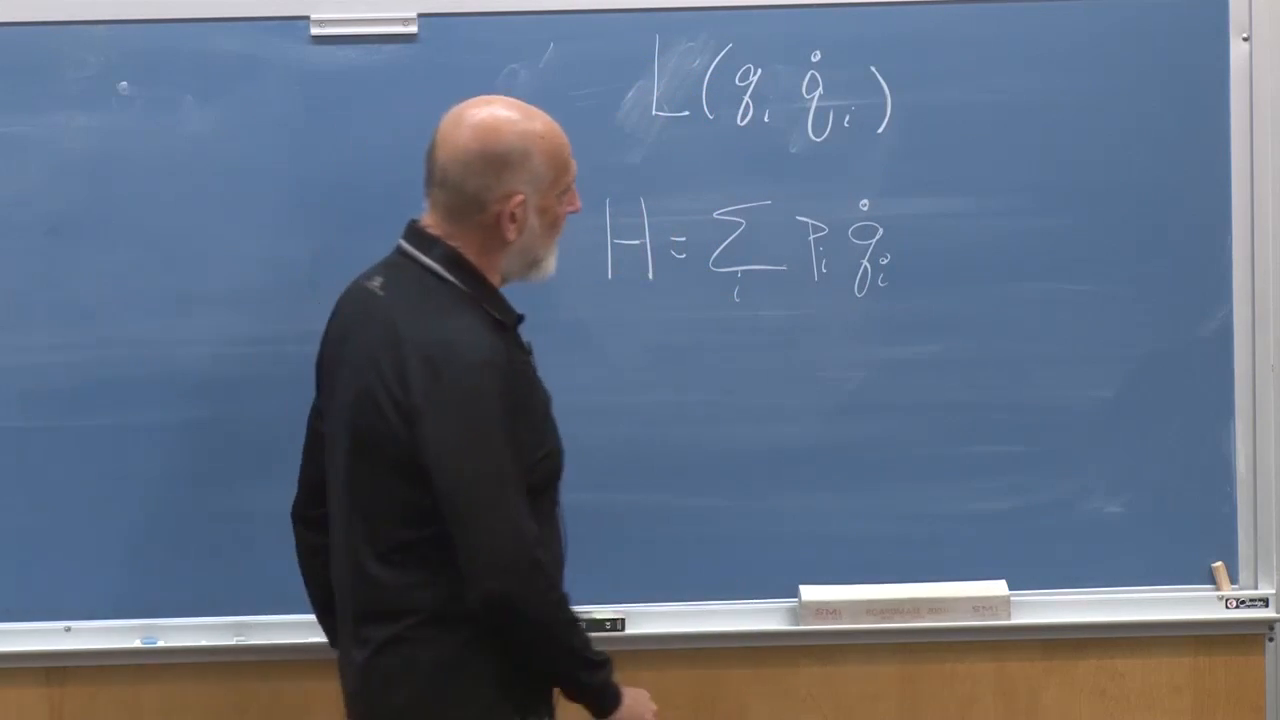
\includegraphics[width=\linewidth]{lecture_10_figure_06.png}
\caption{将哈密顿量写为一般拉格朗日量的勒让德变换。}
\par\smallskip
\textit{授课画面：00:22:55。}
\end{figure}

对于单粒子例子，
\begin{align}
p&=m\dot x,
\nonumber\\
H&=p\dot x-L\\
&=m\dot x^2
  -\left(\frac12m\dot x^2-V(x)\right)\\
&=\frac12m\dot x^2+V(x).
\label{eq:particle-hamiltonian}
\end{align}
因此拉格朗日量是动能减势能，而哈密顿量是动能加势能。

\begin{figure}[H]
\centering
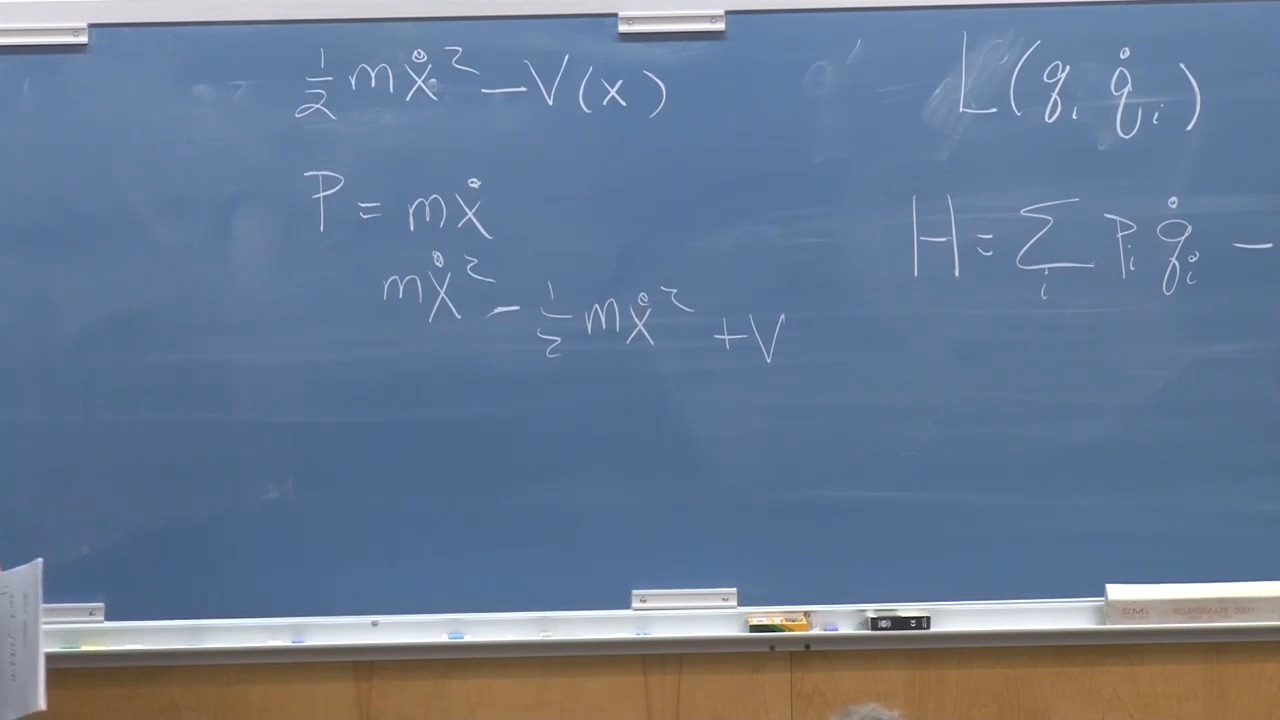
\includegraphics[width=\linewidth]{lecture_10_figure_07.png}
\caption{粒子计算展示了\(H=T+V\)如何由\(H=p\dot x-L\)得出。}
\par\smallskip
\textit{授课画面：00:24:20。}
\end{figure}

当所有速度依赖都是常规的正二次动能项，而其余部分不含速度时，可以通过反转非速度部分的符号来读出哈密顿量。这个捷径将被反复使用。它之所以安全，仅仅是因为在所讨论的例子中勒让德变换具有这种简单形式。

\section{场是一个具有连续多个坐标的力学系统}

为了揭示场论的力学结构，选择一个惯性系，并暂时不再坚持每一行都显示明显的洛伦兹协变性。经典力学有一个时间轴和坐标\(q_i(t)\)。标量场有一个时间轴和坐标\(\phi(\mathbf x,t)\)。离散标签\(i\)只是变成了连续标签\(\mathbf x\)：
\begin{equation}
q_i(t)\quad\longrightarrow\quad\phi(\mathbf x,t).
\label{eq:discrete-to-field}
\end{equation}
场在每个空间点处的值是一个自由度。这里\(\mathbf x\)标记的是所指的自由度；它本身并不是广义坐标。

\begin{figure}[H]
\centering
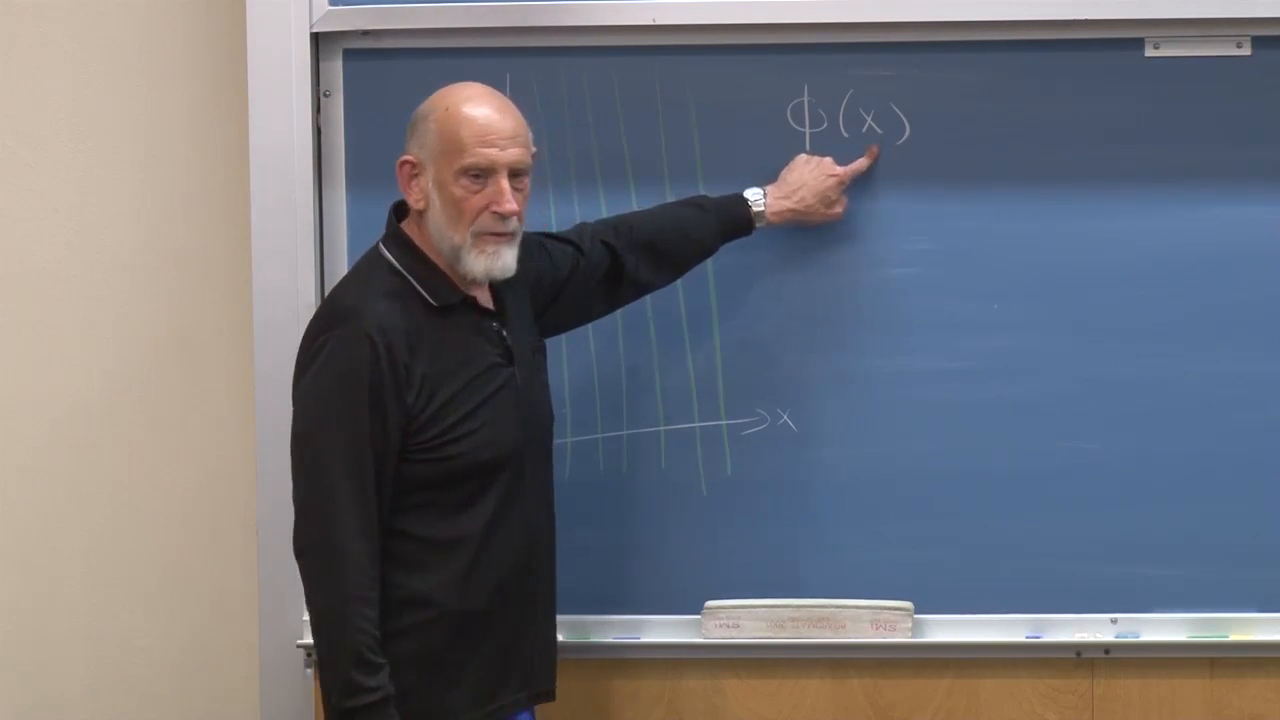
\includegraphics[width=\linewidth]{lecture_10_figure_08.png}
\caption{用空间点阵将每个点处的场值显示为独立的力学自由度。}
\par\smallskip
\textit{授课画面：00:30:15。}
\end{figure}

\begin{classroomqa}
\audiencequestion{为什么不从一开始就把场写成
\(\phi(\mathbf x,t)\)？}
\lecturerresponse{那是完整的记号。临时的
\(\phi(\mathbf x)\)省略了共同的时间自变量，就像人们常写\(q_i\)而记住每个\(q_i\)都依赖于时间一样。标签\(i\)，或者现在的\(\mathbf x\)，告诉我们正在讨论的是哪个自由度。\lecturetimestamp{00:32:43}}
\end{classroomqa}

\begin{classroomqa}
\audiencequestion{相邻点处的场值真的是独立坐标吗？是什么施加了连续性？}
\lecturerresponse{它们是独立的正则坐标。光滑性不是通过把相邻值等同起来而施加的；它是动力学地选择出来的。哈密顿量包含一个正的梯度能量项，因此在越来越小的距离上保持固定的跳变会花费越来越多的能量。因此，在连续极限下，有限能量的构型是光滑的。\lecturetimestamp{00:33:09}}
\end{classroomqa}

空间导数使相邻自由度之间的耦合变得明确。在间距为\(\epsilon\)的点阵上，
\begin{equation}
\partial_x\phi(x,t)
  =\lim_{\epsilon\to0}
   \frac{\phi(x+\epsilon,t)-\phi(x,t)}{\epsilon}.
\label{eq:field-finite-difference}
\end{equation}
它依赖于两个邻近坐标，但不包含广义速度。在力学类比中，它属于拉格朗日量的坐标依赖，而不属于\(\dot q_i\)依赖。

\begin{figure}[H]
\centering
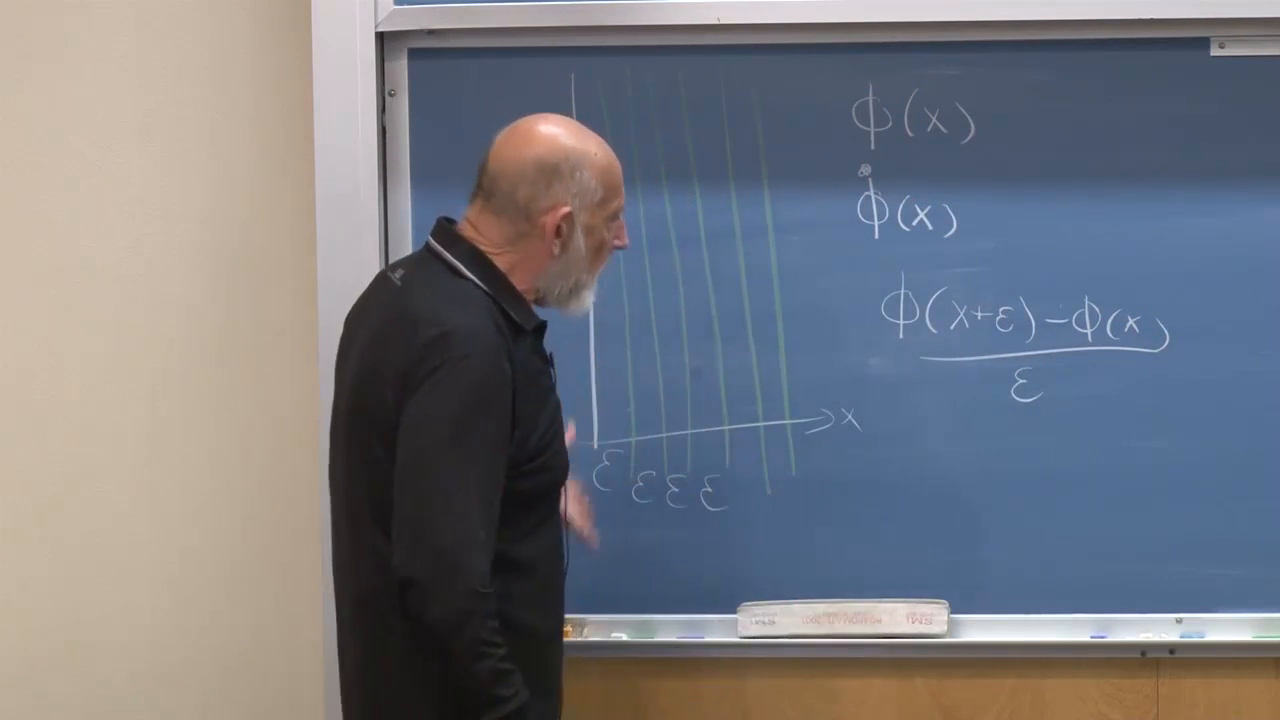
\includegraphics[width=\linewidth]{lecture_10_figure_09.png}
\caption{将空间导数重建为点阵上的相邻场之差。}
\par\smallskip
\textit{授课画面：00:31:40。}
\end{figure}

作用量现在可以写成显式的力学形式：
\begin{align}
S&=\int dt\,L,
\nonumber\\
L&=\int d^3x\,
\mathcal L\!\left(
\phi,\dot\phi,\boldsymbol{\nabla}\phi
\right),
\nonumber\\
S&=\int dt\,d^3x\,
\mathcal L\!\left(
\phi,\dot\phi,\boldsymbol{\nabla}\phi
\right).
\label{eq:field-action-split}
\end{align}
花体字母\(\mathcal L\)是拉格朗日密度；将其对空间积分给出对时间积分的普通拉格朗日量。局域理论只通过该点处的场及其导数来耦合每个点。将时间与空间分开会暂时隐藏洛伦兹协变性，但使力学变得透明。

\begin{figure}[H]
\centering
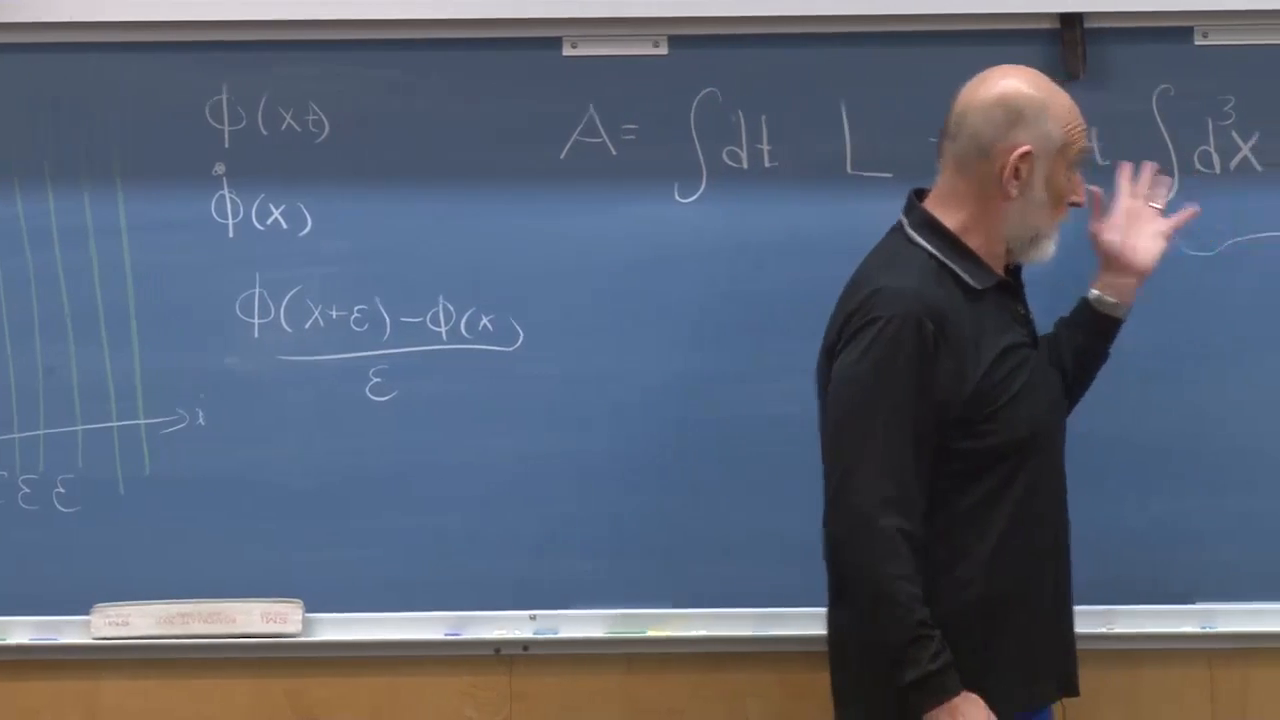
\includegraphics[width=\linewidth]{lecture_10_figure_10.png}
\caption{场作用量分解为对拉格朗日密度的时间积分与空间积分。}
\par\smallskip
\textit{讲义帧：00:36:40。}
\end{figure}

\section{正则场动量与哈密顿密度}

场坐标的速度是\(\dot\phi(\mathbf x,t)\)：即场在某一固定点处随时间变化的速率。它不是从一个空间点运动到另一个空间点。因此，与场共轭的正则动量本身也是一个场，
\begin{equation}
\Pi(\mathbf x,t)
 =\frac{\partial\mathcal L}{\partial\dot\phi(\mathbf x,t)}.
\label{eq:field-canonical-momentum}
\end{equation}
对于多个场\(\phi_a\)，每一个都有一个动量场\(\Pi_a\)。

勒让德变换中的离散求和变为空间积分：
\begin{align}
H
 &=\int d^3x\,
   \left[\Pi\dot\phi-\mathcal L\right]
  =\int d^3x\,\mathcal H,
\nonumber\\
\mathcal H
 &=\Pi\dot\phi-\mathcal L .
\label{eq:field-hamiltonian-density}
\end{align}
积分内的量就是能量密度。

\begin{figure}[H]
\centering
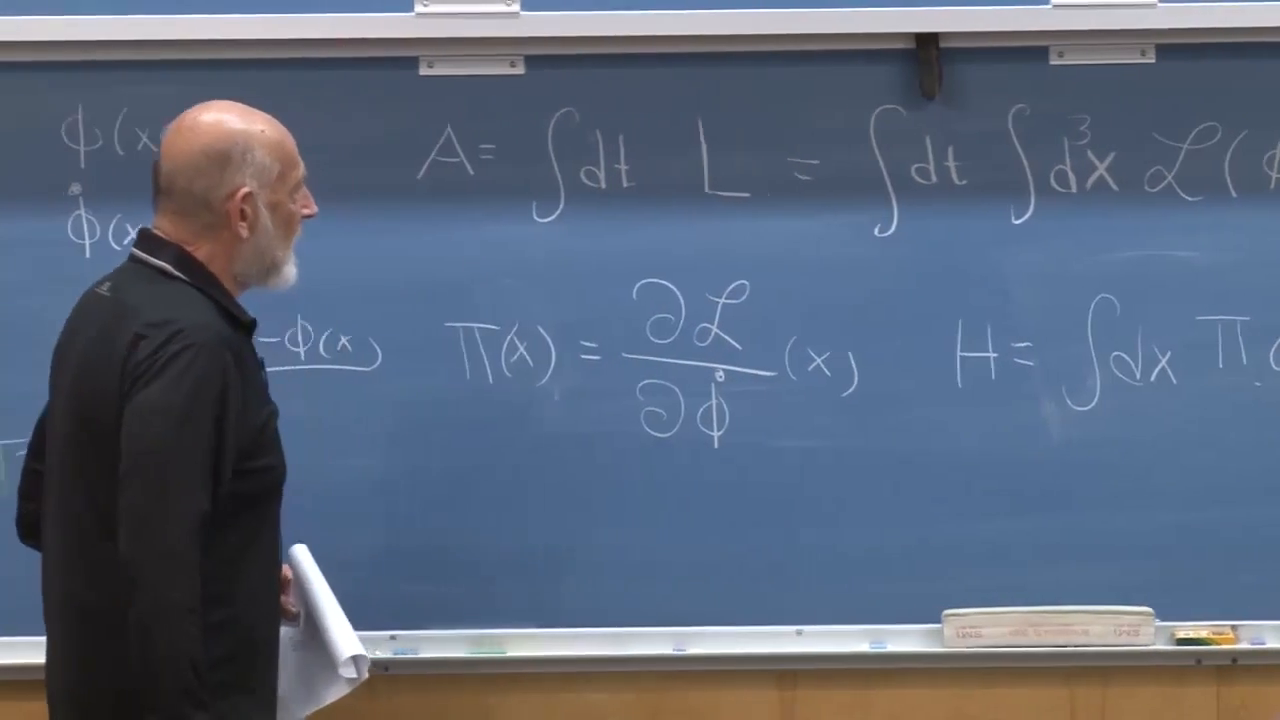
\includegraphics[width=\linewidth]{lecture_10_figure_11.png}
\caption{场的勒让德变换及其解释为局域能量密度的积分。}
\par\smallskip
\textit{讲义帧：00:42:40。}
\end{figure}

\begin{classroomqa}
\audiencequestion{为什么总拉格朗日量对某一点处\(\dot\phi\)的导数可以替换为该点处局域密度的导数？}
\lecturerresponse{把空间积分看作连续求和。
在此处所用的局域性假设下，速度
\(\dot\phi(\mathbf x)\)只出现在属于同一点的那一项中。对该特定速度求导会消去所有其他项。空间导数可能耦合相邻的场值，但在这个理论中它们不会引入相邻的时间导数。\lecturetimestamp{00:51:56}}
\end{classroomqa}

\subsection{标量场}

在一维空间中，取
\begin{equation}
\mathcal L
 =\frac12\dot\phi^2
  -\frac12(\partial_x\phi)^2
  -V(\phi).
\label{eq:scalar-field-lagrangian}
\end{equation}
这是前面用过的洛伦兹标量的非协变写法：时间导数与空间导数之间的相对负号来自闵可夫斯基度规。正则动量为
\begin{equation}
\Pi=\dot\phi,
\label{eq:scalar-pi}
\end{equation}
而哈密顿量变为
\begin{equation}
H=\int dx\,
\left[
\frac12\dot\phi^2
+\frac12(\partial_x\phi)^2
+V(\phi)
\right].
\label{eq:scalar-field-hamiltonian}
\end{equation}
在计算过程中，势曾被暂时称为\(V(x)\)；班上把它改正为\(V(\phi)\)。它可以通过场间接依赖于位置，但在平移不变理论中，它没有指定的外部\(x\)依赖性。

\begin{figure}[H]
\centering
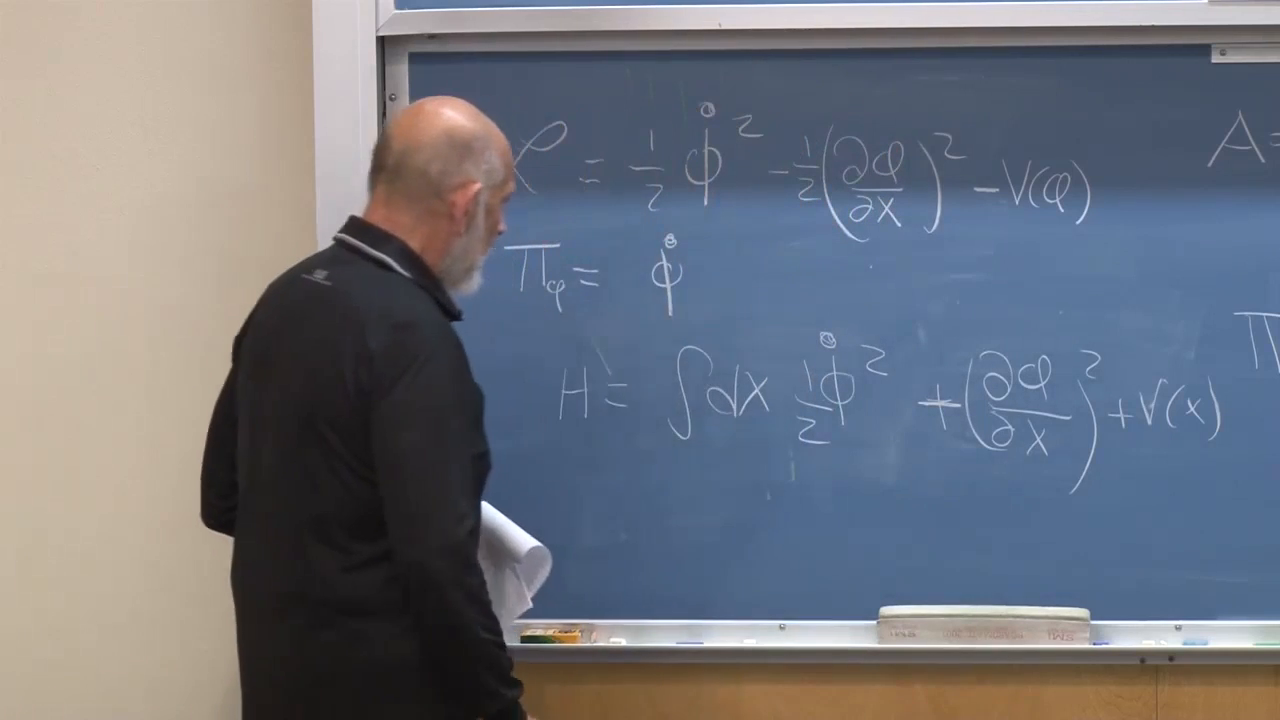
\includegraphics[width=\linewidth]{lecture_10_figure_12.png}
\caption{标量拉格朗日密度、共轭动量与正定哈密顿量汇集在一块黑板上。}
\par\smallskip
\textit{讲义帧：00:47:05。}
\end{figure}

不含时间导数的整个部分起势能的作用。这既包括\(V(\phi)\)，也包括梯度能量\(\frac12(\partial_x\phi)^2\)。拉格朗日量可以取任一种符号；稳定的能量应当有下界。

\begin{classroomqa}
\audiencequestion{势\(V(\phi)\)可以为负吗？}
\lecturerresponse{可以。如果它有有限下界，可以加上一个常数使其最小值为零，而不改变经典场方程。无下界的势描述一种不稳定性：场可以无限制地降低其能量。稳定真空是位于平移后势的极小值处的常场。
\lecturetimestamp{00:49:03}}
\end{classroomqa}

先前的连续性问题现在得到了定量回答。跨越点阵间距\(\epsilon\)的跳变\(\Delta\phi\)贡献
\begin{equation}
\frac12(\partial_x\phi)^2
\sim\frac12\left(\frac{\Delta\phi}{\epsilon}\right)^2.
\label{eq:gradient-cost}
\end{equation}
当\(\epsilon\to0\)时，固定的跳变给出任意大的能量密度。因此有限能量会抑制锯齿状构型。

\begin{figure}[H]
\centering
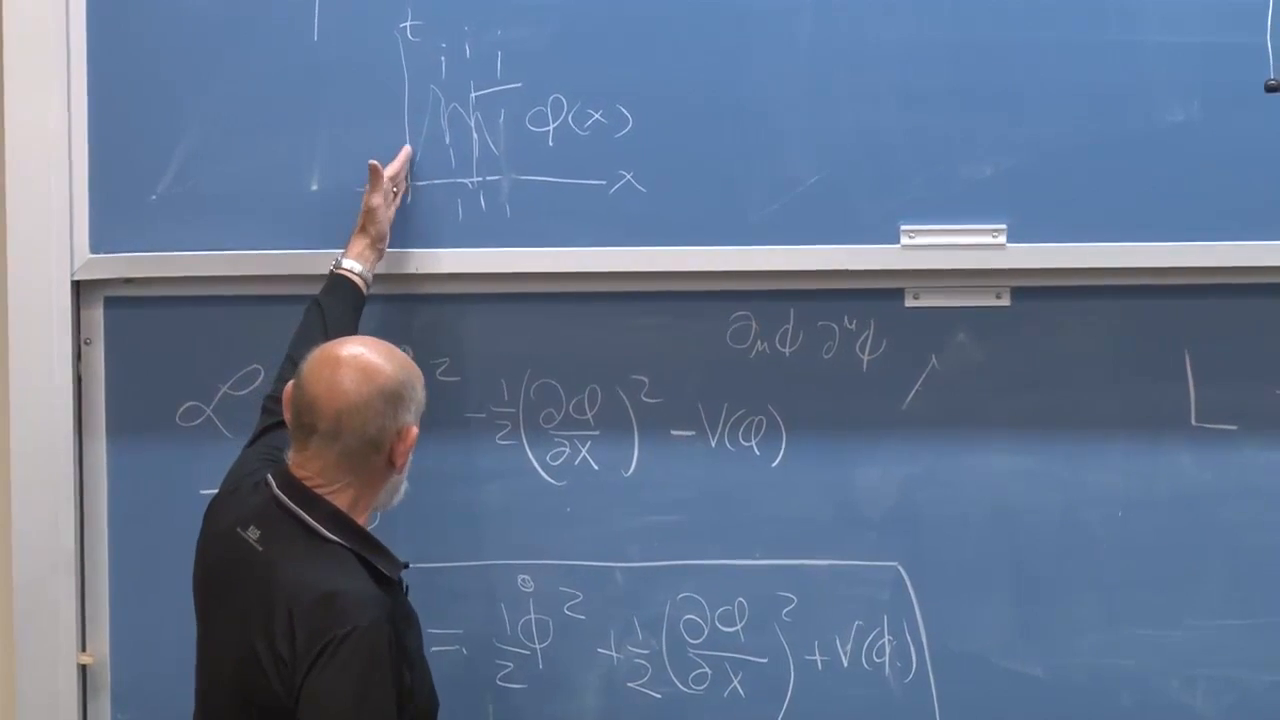
\includegraphics[width=\linewidth]{lecture_10_figure_13.png}
\caption{保留标量能量公式，同时黑板草图将光滑场与尖锐变化作对比。}
\par\smallskip
\textit{讲义帧：00:54:20。}
\end{figure}

\section{局部能量与\texorpdfstring{\(T^{00}\)}{T00}的意义}

能量密度获得了一个简洁的名称：
\begin{equation}
T^{00}=\mathcal H=\Pi\dot\phi-\mathcal L.
\label{eq:T00-definition}
\end{equation}
两个零指标编码了两个不同的陈述。能量是能量--动量四矢量的时间分量\(P^0\)，而密度是守恒流的时间分量。因此\(T^{00}\)是四动量时间分量的密度。

\begin{figure}[H]
\centering
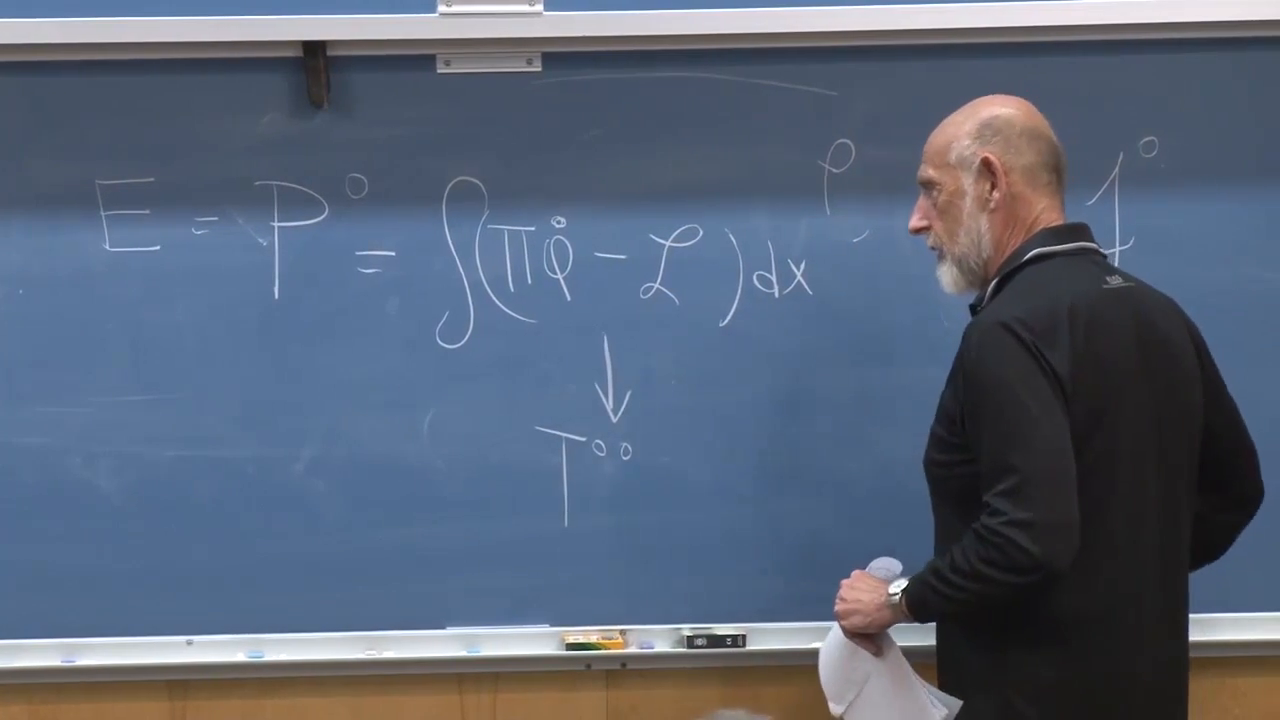
\includegraphics[width=\linewidth]{lecture_10_figure_14.png}
\caption{局域写出的场能量，并等同于\(T^{00}\)。}
\par\smallskip
\textit{讲义帧：01:00:00。}
\end{figure}

相对论性局域理论中的守恒不仅仅是一个全局数保持不变的陈述。能量不可能在实验室中消失并在半人马座{\proseunicodefont α}重新出现。一个区域内部的变化必须由穿过其边界的通量来解释。以局域形式，
\begin{equation}
\partial_\mu T^{\mu\nu}=0,
\label{eq:stress-energy-continuity}
\end{equation}
因此第一个指标标记密度或通量方向，第二个指标标记正在被输运的是哪个分量\(P^\nu\)。

\begin{classroomqa}
\audiencequestion{把\(T^{00}\)称为密度，是否意味着总能量要通过对它积分来得到？}
\lecturerresponse{正是如此：\(E=P^0=\int d^3x\,T^{00}\)。局域密度就是场论勒让德变换中的被积函数。它在某一处的变分由穿过邻近各处的能量流所平衡。\lecturetimestamp{00:59:06}}
\end{classroomqa}

\section{由空间平移得到的动量密度}

回到诺特定理的公式，现在把离散求和替换为空间积分。在沿\(m\)方向的小平移下，按照黑板上采用的被动约定，场的变化为
\begin{equation}
\delta\phi
  =\phi(\mathbf x)-\phi(\mathbf x-\boldsymbol{\epsilon})
  =\epsilon^m\partial_m\phi+O(\epsilon^2),
\label{eq:translated-field-change}
\end{equation}
交换主动平移与被动平移会反转整体符号；一旦选定了该约定，物理的生成元就确定了。提出\(\epsilon^m\)后，诺特动量具有如下结构
\begin{equation}
P_m\ \propto\ \int d^3x\,\Pi\,\partial_m\phi.
\label{eq:scalar-noether-momentum}
\end{equation}

\begin{figure}[H]
\centering
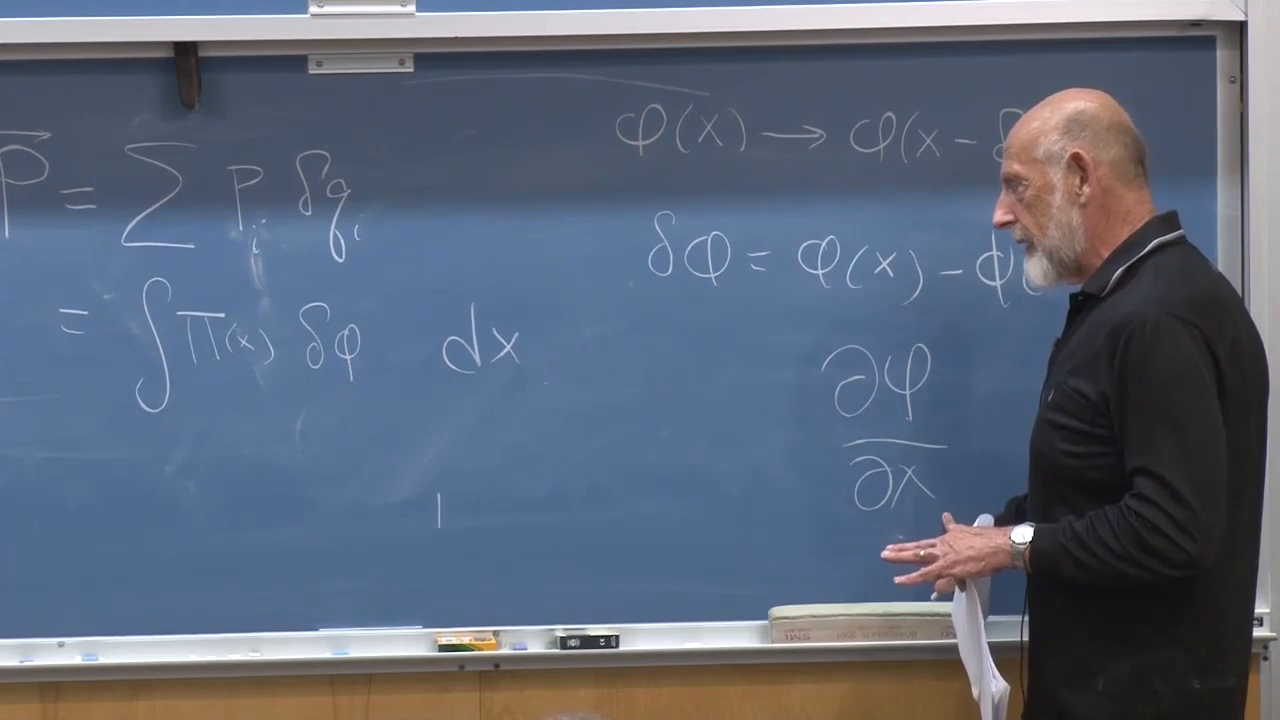
\includegraphics[width=\linewidth]{lecture_10_figure_15.png}
\caption{平移后的场剖面，以及度量其无穷小变化的导数。}
\par\smallskip
\textit{讲课画面：01:04:20。}
\end{figure}

\begin{classroomqa}
\audiencequestion{为什么无穷小平移\(\epsilon\)没有保留在动量公式中？}
\lecturerresponse{诺特荷最初得到时正比于\(\epsilon\)。动量被定义为那个任意平移参数的系数，因此\(\epsilon\)被除掉了。把一个守恒量乘以固定常数不会影响守恒性，但提取系数才能给出标准归一化。\lecturetimestamp{01:04:45}}
\end{classroomqa}

\begin{classroomqa}
\audiencequestion{平移间隔会变成连续积分中的\(dx\)吗？}
\lecturerresponse{它们来自不同的极限。测度\(dx\)来自把对带空间标签的自由度的求和替换为积分。平移参数\(\epsilon\)描述对称操作，并从其诺特荷中提出。二者在中间推理中都是无穷小量，但它们扮演的角色不同。\lecturetimestamp{01:05:16}}
\end{classroomqa}

按照讲课中的记号，动量\(m\)分量的密度为
\begin{equation}
T^{0m}=\Pi\,\partial_m\phi,
\label{eq:scalar-momentum-density}
\end{equation}
其中隐含了平移符号约定。对于标量理论，\(\Pi=\dot\phi\)，因此它正比于\(\dot\phi\,\partial_m\phi\)。

\begin{figure}[H]
\centering
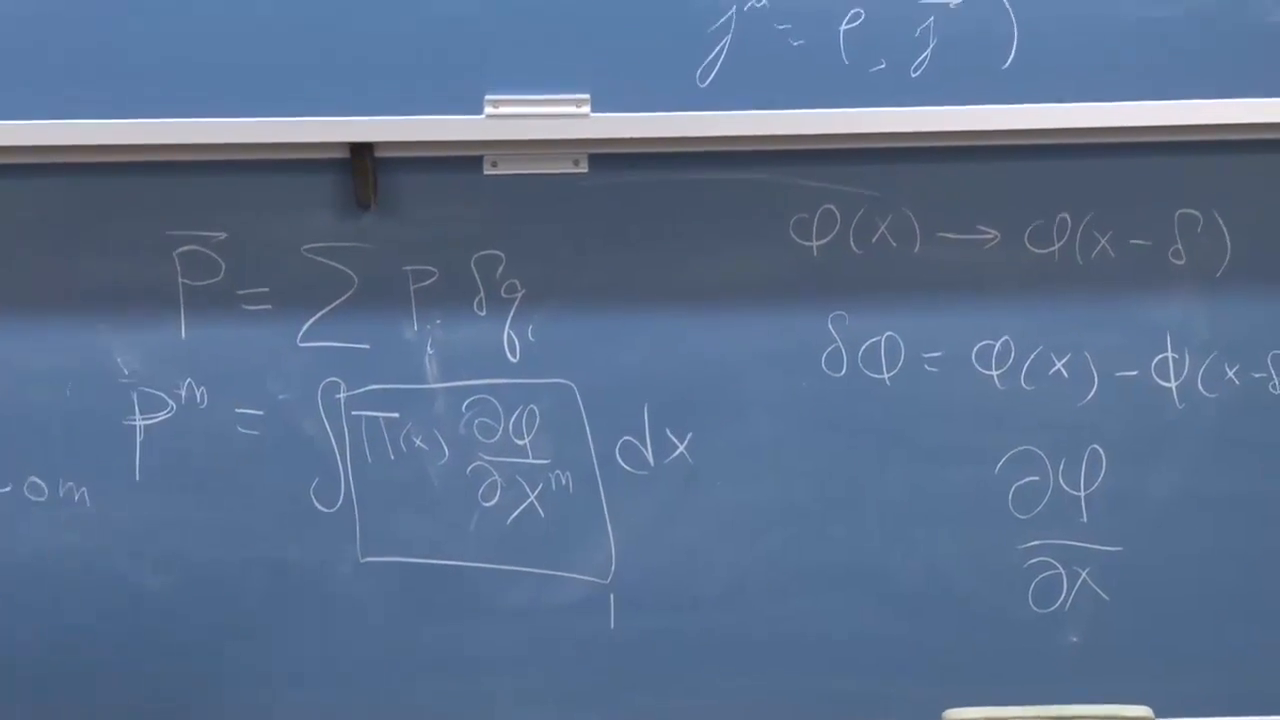
\includegraphics[width=\linewidth]{lecture_10_figure_16.png}
\caption{黑板上的诺特动量密度\(T^{0m}=\Pi\,\partial_m\phi\)。}
\par\smallskip
\textit{讲课画面：01:07:10。}
\end{figure}

这就是波所携带的真正的动量。平移不变性只有在一切都被平移时才成立：场、粒子、源和仪器。被自由悬挂的板吸收的光脉冲会给板一个反冲。普通光使这一效应极其微小；足够强的激光可以传递足够的动量来压缩一个小靶。守恒的总量属于粒子和场共同所有。

\subsection{什么取代了牛顿方程？}

由式~\eqref{eq:scalar-field-lagrangian}导出的场欧拉--拉格朗日方程为
\begin{equation}
\ddot\phi-\nabla^2\phi=-\frac{dV}{d\phi}.
\label{eq:scalar-equation-of-motion}
\end{equation}
它是牛顿定律在场论中的对应物。

\begin{figure}[H]
\centering
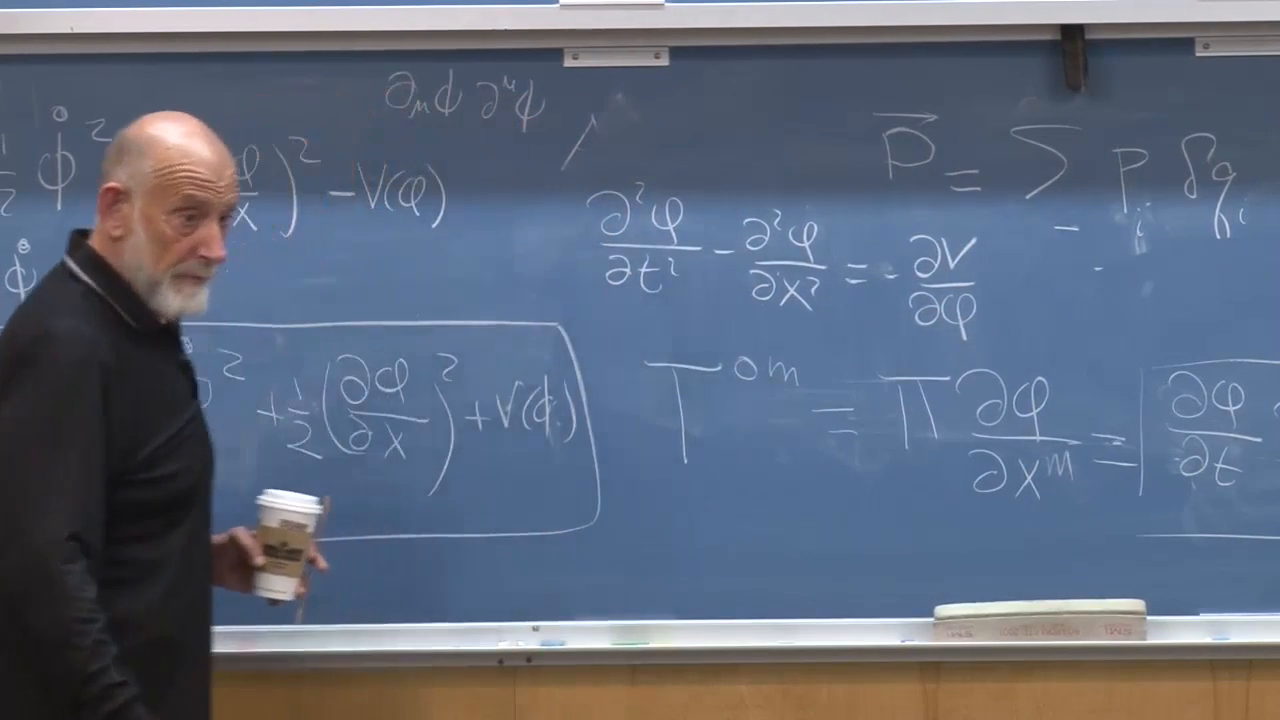
\includegraphics[width=\linewidth]{lecture_10_figure_17.png}
\caption{标量场方程与它的哈密顿量和动量密度并列显示。}
\par\smallskip
\textit{讲课画面：01:12:55。}
\end{figure}

\begin{classroomqa}
\audiencequestion{对于场而言，什么对应于牛顿定律？}
\lecturerresponse{欧拉--拉格朗日场方程与之对应。这里它是一个带有力项\(-V'(\phi)\)的波动方程。\(m\ddot x=-V'(x)\)的角色由\(\ddot\phi-\nabla^2\phi=-V'(\phi)\)扮演。
\lecturetimestamp{01:11:48}}
\end{classroomqa}

\begin{classroomqa}
\audiencequestion{我们怎么知道一个提出的场拉格朗日量是正确的？我们必须已经知道场方程吗？}
\lecturerresponse{两个方向都有可能。历史上，人们可以从实验推断方程，然后寻找作用量，牛顿和麦克斯韦的情形就是如此。在现代理论中，人们常常从场的内容、局域性、对称性以及一小组可允许的项出发，导出方程，并检验其预言。所展示的标量场可以描述一个基本场，但它同样可以描述一根绳子的横向位移，而该绳子的连续作用量是由其组成粒子导出的。\lecturetimestamp{01:12:55}}
\end{classroomqa}

\section{时间规范下的电磁场}

已经找到的分量\(T^{00}\)和\(T^{0m}\)属于能量--动量张量。它的其余分量描述能量和动量通量。这个张量以后将作为引力的源，但电磁学提供了眼前的例子。

基本的电磁坐标是四维势 \(A_\mu\)。
规范自由度允许
\begin{equation}
A_\mu\longrightarrow A'_\mu=A_\mu+\partial_\mu S
\label{eq:gauge-transformation-lecture10}
\end{equation}
而不改变 \(F_{\mu\nu}\)。选择 \(S\) 使其满足
\begin{equation}
\partial_tS=-A_0.
\label{eq:temporal-gauge-choice}
\end{equation}
例如，可以在每个固定的空间点上对 \(A_0\) 进行时间积分。变换后的时间分量随即消失：
\begin{equation}
A'_0=A_0+\partial_tS=0.
\label{eq:temporal-gauge}
\end{equation}
这就是时间规范。它把 \(A_0\) 从动力学坐标的列表中移除，尽管高斯定律仍作为约束保留下来，并且还残留一个与时间无关的剩余规范自由度。

\begin{figure}[H]
\centering
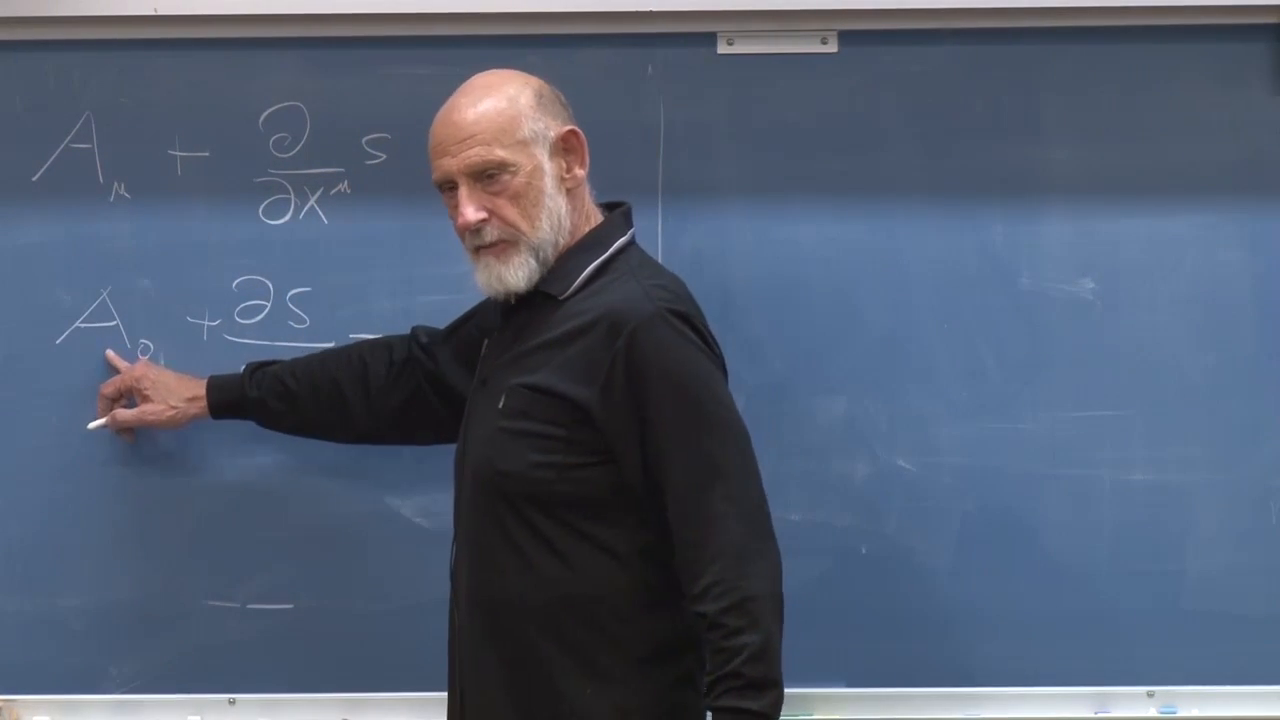
\includegraphics[width=\linewidth]{lecture_10_figure_18.png}
\caption{利用规范自由度，通过求解 \(\partial_tS=-A_0\) 来选择 \(A_0=0\)。}
\par\smallskip
\textit{讲义帧：01：20：15。}
\end{figure}

从现在起，令 \(\mathbf E\) 表示标准的麦克斯韦场。在规范固定之前，
\begin{equation}
E_m=-\partial_tA_m+\partial_mA_0,
\qquad
\mathbf B=\boldsymbol{\nabla}\times\mathbf A.
\label{eq:E-B-general-potential}
\end{equation}
在时间规范下，这些关系简化为
\begin{equation}
\mathbf E=-\dot{\mathbf A},
\qquad
\mathbf B=\boldsymbol{\nabla}\times\mathbf A.
\label{eq:E-B-temporal-gauge}
\end{equation}
\(\mathbf A\) 的时间导数产生电场；空间导数产生磁场。

\begin{figure}[H]
\centering
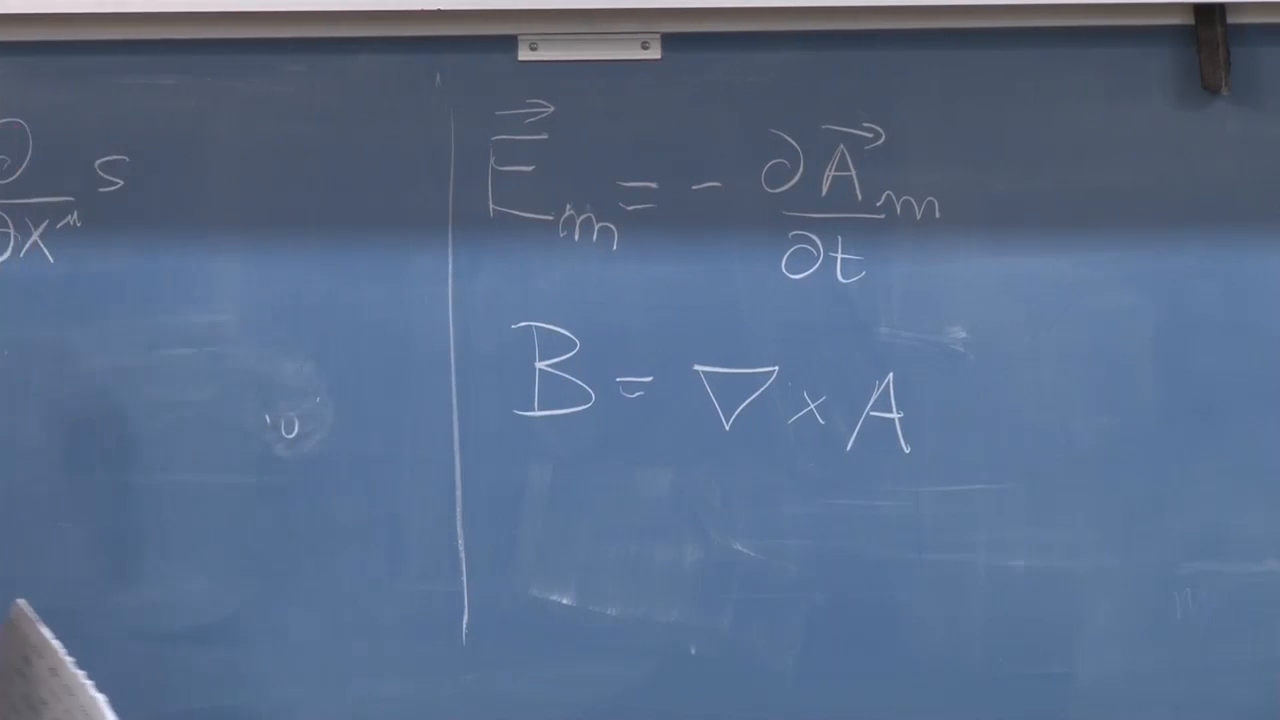
\includegraphics[width=\linewidth]{lecture_10_figure_19.png}
\caption{时间规范下的电场和磁场：
\(\mathbf E=-\dot{\mathbf A}\) 和
\(\mathbf B=\nabla\times\mathbf A\)。}
\par\smallskip
\textit{讲义帧：01：23：50。}
\end{figure}

\section{电磁正则动量与能量}

自由麦克斯韦拉格朗日密度为
\begin{equation}
\mathcal L_{\mathrm{EM}}
 =-\frac14F_{\mu\nu}F^{\mu\nu}
 =\frac12\left(\mathbf E^2-\mathbf B^2\right).
\label{eq:maxwell-lagrangian-energy-lecture}
\end{equation}
在时间规范下，
\begin{equation}
\mathcal L_{\mathrm{EM}}
 =\frac12\dot{\mathbf A}^{\,2}
  -\frac12(\boldsymbol{\nabla}\times\mathbf A)^2.
\label{eq:maxwell-lagrangian-temporal}
\end{equation}
它恰好具有标量场的模式：时间导数的平方减去空间导数的平方。

\begin{figure}[H]
\centering
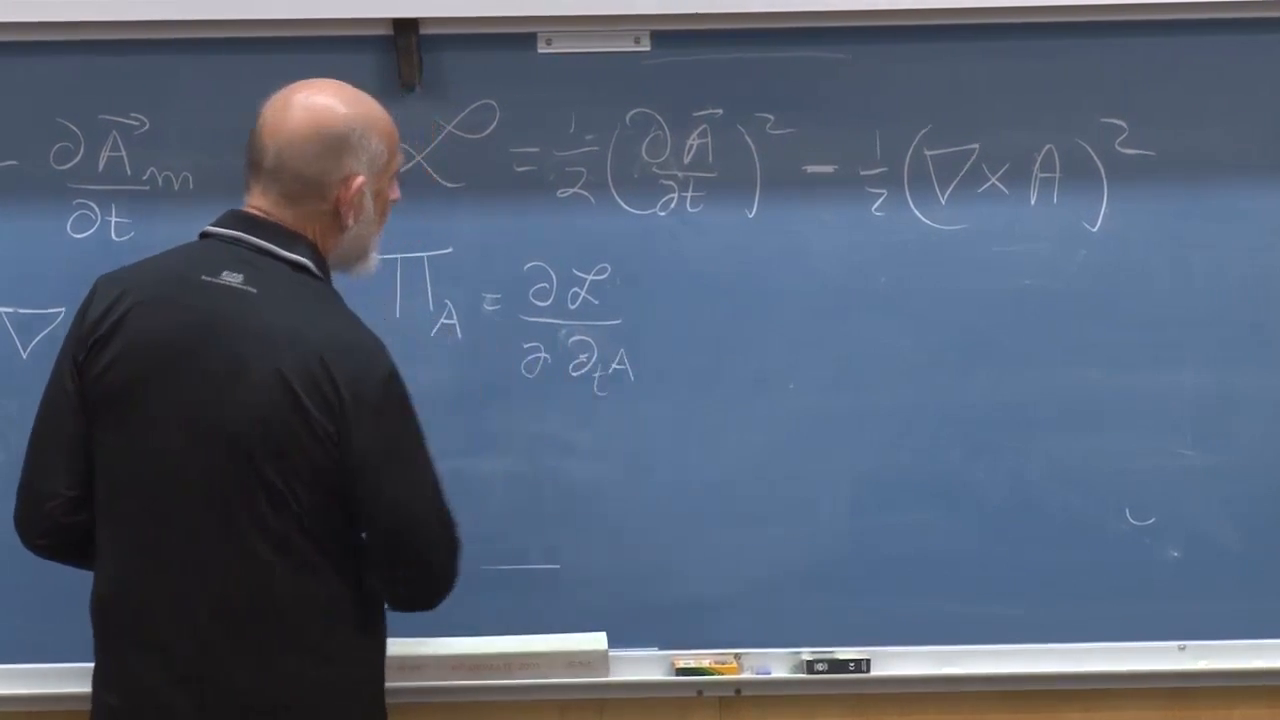
\includegraphics[width=\linewidth]{lecture_10_figure_20.png}
\caption{将麦克斯韦拉格朗日量改写为 \(\mathbf A\) 的空间分量的力学场拉格朗日量。}
\par\smallskip
\textit{讲义帧：01：28：10。}
\end{figure}

每个分量 \(A_m\) 都有一个正则动量，
\begin{equation}
\Pi_m
 =\frac{\partial\mathcal L_{\mathrm{EM}}}
        {\partial\dot A_m}
 =\dot A_m
 =-E_m.
\label{eq:em-canonical-momentum}
\end{equation}
这是一个具体的例子，说明为什么约定很重要。在先前相反的电场约定中，最终显示的符号会改变，尽管正则导数本身不会改变。

\begin{figure}[H]
\centering
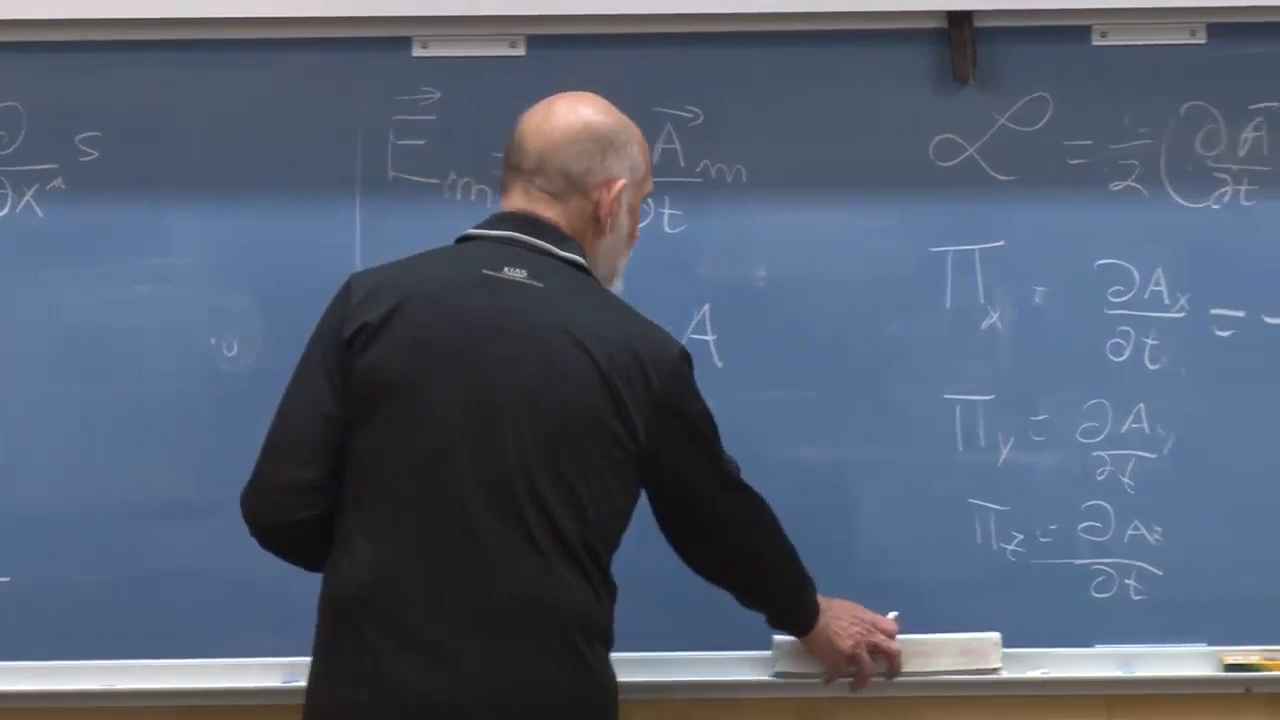
\includegraphics[width=\linewidth]{lecture_10_figure_21.png}
\caption{与 \(A_x,A_y,A_z\) 相关联的三个正则动量场，每一个都等于相应的时间导数，因此等于标准电场的负值。}
\par\smallskip
\textit{讲义帧：01：30：20。}
\end{figure}

现在可以证明哈密顿量捷径是合理的：将非时间导数项的符号反转。电磁能量密度为
\begin{equation}
T^{00}_{\mathrm{EM}}
 =\mathcal H_{\mathrm{EM}}
 =\frac12\left(\mathbf E^2+\mathbf B^2\right),
\label{eq:em-energy-density}
\end{equation}
以及
\begin{equation}
H_{\mathrm{EM}}
 =\int d^3x\,
\frac12\left(\mathbf E^2+\mathbf B^2\right).
\label{eq:em-total-energy}
\end{equation}
与拉格朗日密度不同，能量密度是非负的。

\begin{figure}[H]
\centering
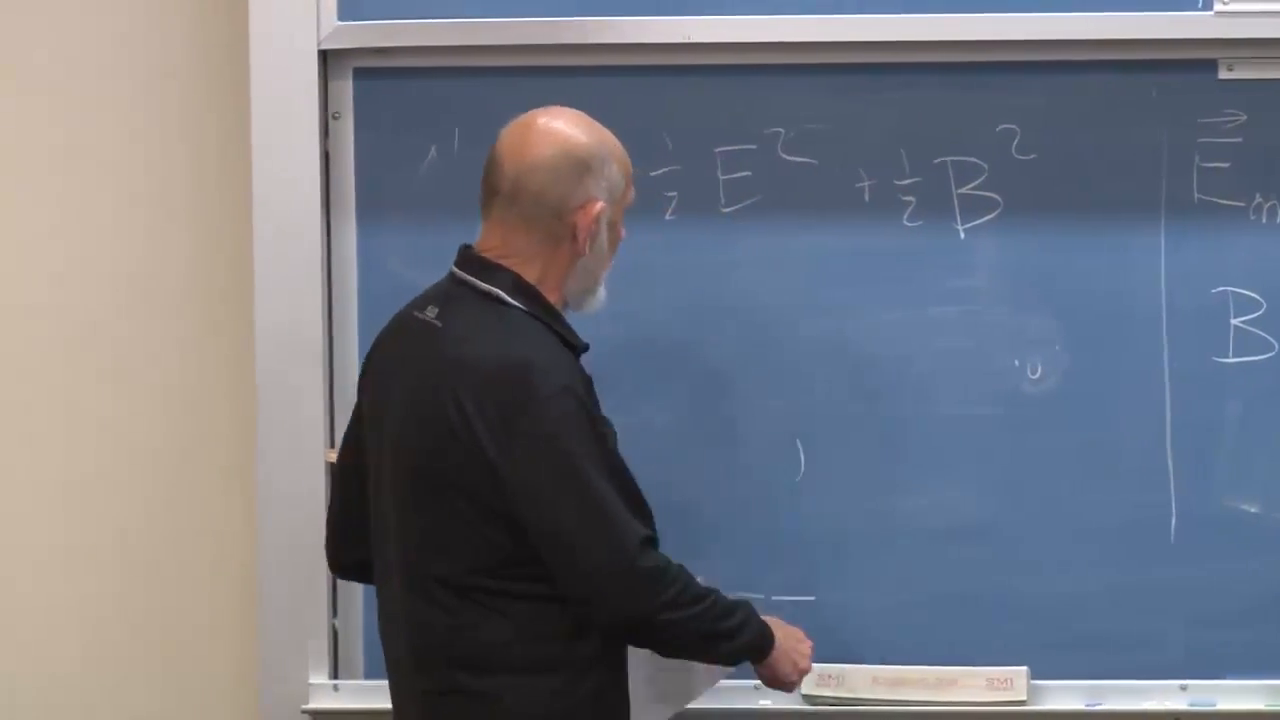
\includegraphics[width=\linewidth]{lecture_10_figure_22.png}
\caption{正的电磁哈密顿量密度 \(\frac12(\mathbf E^2+\mathbf B^2)\)。}
\par\smallskip
\textit{讲义帧：01：32：00。}
\end{figure}

对于真空中的平面波，\(\mathbf E\perp\mathbf B\)，这两个场同相，并且在 \(c=1\) 单位下它们大小相等。因此电场和磁场的贡献平分波的能量：
\begin{equation}
u_E=\frac12\mathbf E^2,
\qquad
u_B=\frac12\mathbf B^2,
\qquad
u_E=u_B.
\label{eq:plane-wave-energy-halves}
\end{equation}

\section{推导电磁动量}

诺特定理的平移公式现在必须对三个场 \(A_m\) 求和。选择平移符号使得物理动量指向波传播方向，则 \(n\) 分量为
\begin{equation}
P_n
 =\int d^3x\,E_m\,\partial_nA_m,
\label{eq:em-canonical-noether-momentum}
\end{equation}
其中 \(m\) 被求和。讲义特意在符号上停顿：它取决于先前的电场约定以及主动/被动平移的选择。规范不变的物理结果将确定它。

\begin{figure}[H]
\centering
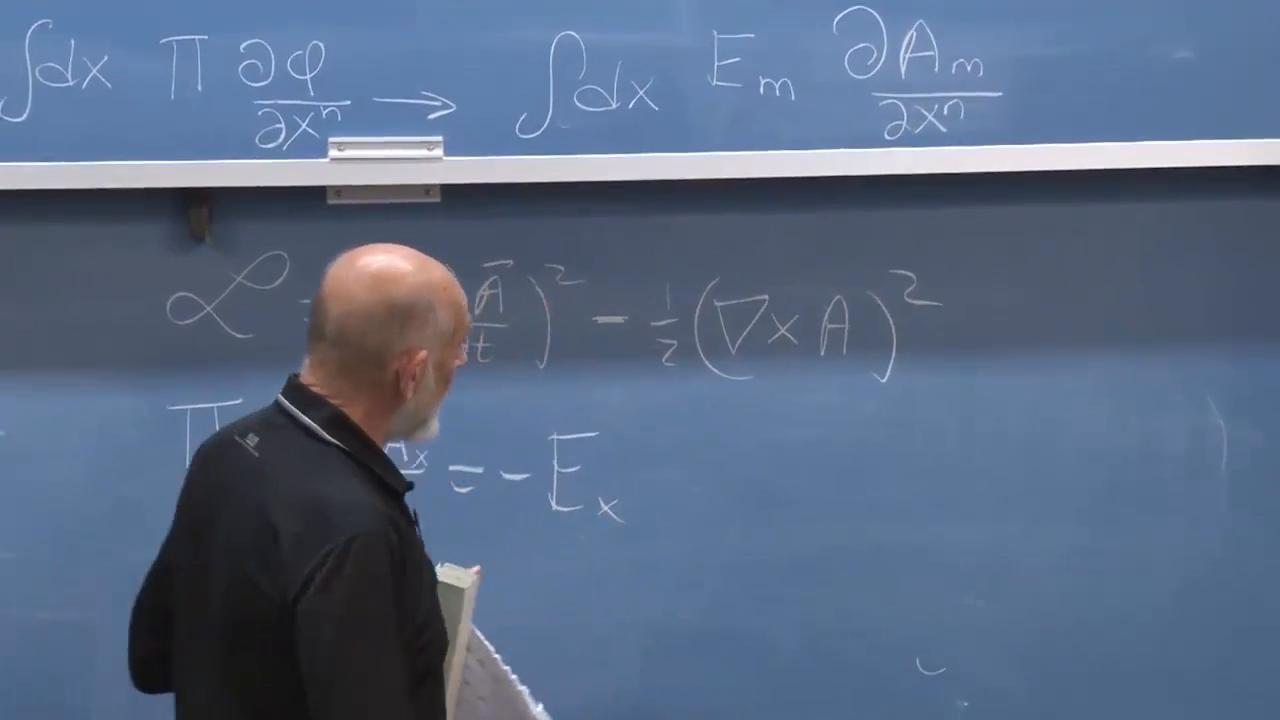
\includegraphics[width=\linewidth]{lecture_10_figure_23.png}
\caption{将标量场的诺特公式推广到矢量势的三个分量。}
\par\smallskip
\textit{讲义帧：01：36：40。}
\end{figure}

被积函数仍然包含规范势，而不仅仅是物理场。插入并减去
\(E_m\partial_mA_n\)：
\begin{align}
E_m\partial_nA_m
 &=
 E_m\left(\partial_nA_m-\partial_mA_n\right)
 +E_m\partial_mA_n.
\label{eq:add-subtract-em-momentum}
\end{align}
第一项是叉积，
\begin{equation}
E_m\left(\partial_nA_m-\partial_mA_n\right)
  =(\mathbf E\times\mathbf B)_n.
\label{eq:cross-product-component}
\end{equation}
第二项通过分部积分：
\begin{align}
\int d^3x\,E_m\partial_mA_n
 &=
\int_{\partial V}d\Sigma_m\,E_mA_n
-\int d^3x\,A_n\partial_mE_m.
\label{eq:em-momentum-integration-parts}
\end{align}
如果场衰减得使边界项消失，并且如果该区域无源，使得
\(\boldsymbol{\nabla}\cdot\mathbf E=0\)，则第二项不贡献任何东西。

\begin{figure}[H]
\centering
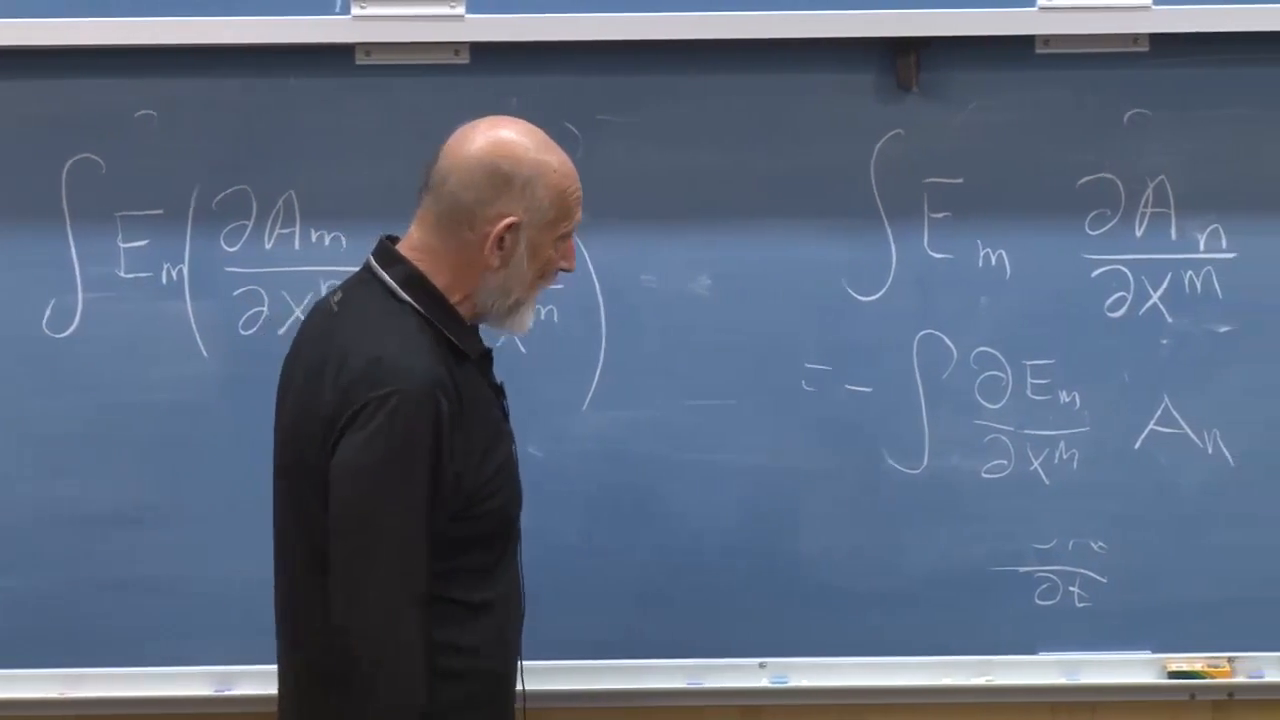
\includegraphics[width=\linewidth]{lecture_10_figure_24.png}
\caption{通过分部积分将添加的项转移到 \(\nabla\cdot\mathbf E\)。}
\par\smallskip
\textit{讲义帧：01：40：00。}
\end{figure}

因此总场动量为
\begin{equation}
\mathbf P_{\mathrm{EM}}
 =\int d^3x\,\mathbf E\times\mathbf B,
\qquad
\mathbf g_{\mathrm{EM}}
 =\mathbf E\times\mathbf B,
\label{eq:em-momentum-density}
\end{equation}
在讲义的各单位下。矢量
\(\mathbf g_{\mathrm{EM}}\) 是电磁动量密度。

\begin{figure}[H]
\centering
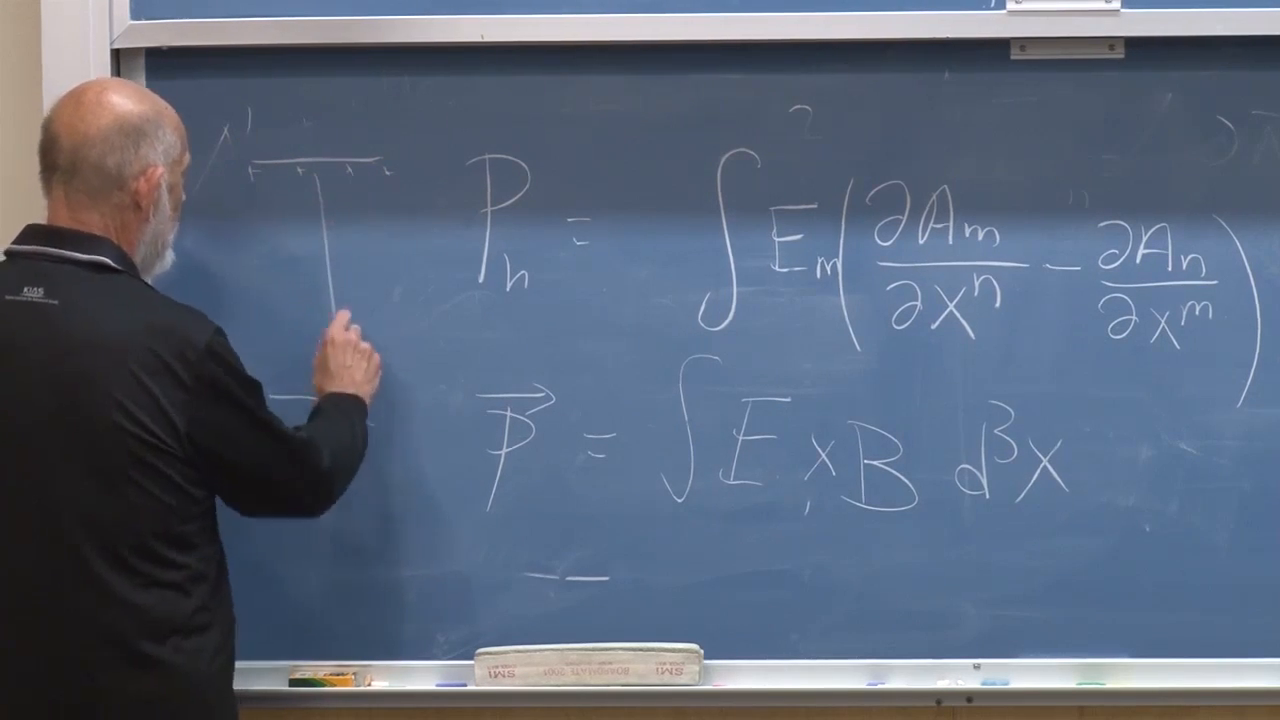
\includegraphics[width=\linewidth]{lecture_10_figure_25.png}
\caption{规范势表达式被约化为规范不变的动量 \(\int d^3x\,\mathbf E\times\mathbf B\)。}
\par\smallskip
\textit{讲义帧：01：41：10。}
\end{figure}

\begin{classroomqa}
\audiencequestion{\(\boldsymbol{\nabla}\cdot\mathbf E=0\)在哪里被用到了，如果存在电荷又会怎样？}
\lecturerresponse{它在分部积分后去掉了体积项，因此所展示的仅含场的推导适用于自由电磁波。存在电荷时，该项不为零，必须把带电物质的动量也包括进来。平移不变性和动量守恒涉及的是完整的物质--场系统。\lecturetimestamp{01:41:55}}
\end{classroomqa}

\subsection{波的方向}

在平面波中，\(\mathbf E\)、\(\mathbf B\)与传播方向构成右手三元组。半个波长之后，\(\mathbf E\)和\(\mathbf B\)都反向：
\begin{equation}
(-\mathbf E)\times(-\mathbf B)
 =\mathbf E\times\mathbf B.
\label{eq:poynting-sign-reversal}
\end{equation}
因此，在整个振荡过程中，动量密度始终指向一个固定方向，即波传播的方向。

\begin{figure}[H]
\centering
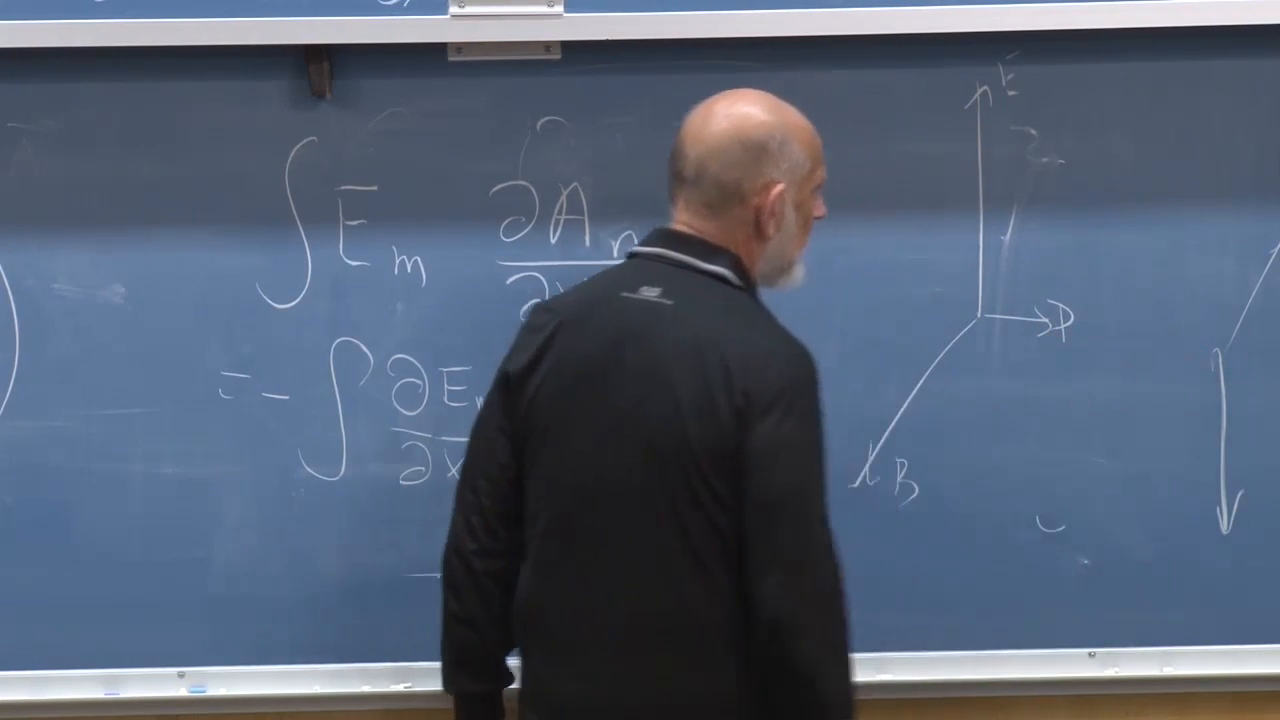
\includegraphics[width=\linewidth]{lecture_10_figure_26.png}
\caption{平面波几何：电场和磁场一起反向，而它们的叉积继续沿传播轴方向。}
\par\smallskip
\textit{课堂画面：01:43:10。}
\end{figure}

这就是光压真实存在的原因。吸收把场的动量传递给物质；反射使光的动量反向，并可以把法向分量的两倍传递给反射体。

\section{势与可观测场相接之处}

在结尾，课堂询问\(A_\mu\)与可观测场之间的接触点。它们正是
\begin{align}
E_n&=-\partial_tA_n+\partial_nA_0,
\nonumber\\
B_n&=\epsilon_{nmk}\partial_mA_k.
\label{eq:potential-field-contact}
\end{align}
时间规范去掉了\(A_0\)项，但不改变物理场。

\begin{figure}[H]
\centering
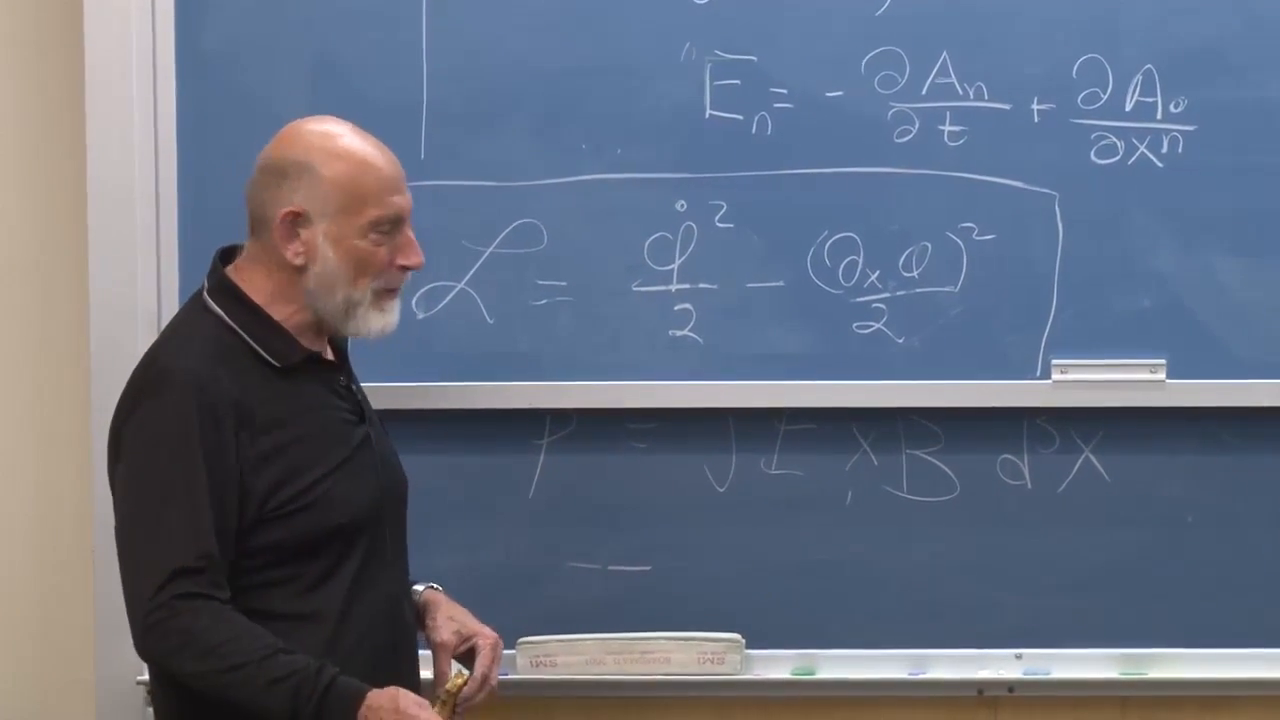
\includegraphics[width=\linewidth]{lecture_10_figure_27.png}
\caption{在时间规范计算之后恢复的一般电场关系，以及其下方回顾的协变标量拉格朗日量。}
\par\smallskip
\textit{课堂画面：01:45:40。}
\end{figure}

\begin{classroomqa}
\audiencequestion{矢量势与电场和磁场究竟在哪里相接？}
\lecturerresponse{电场把空间势的时间导数与\(A_0\)的空间导数结合起来；磁场是空间势的旋度。在时间规范下，这简化为
\(\mathbf E=-\dot{\mathbf A}\)和
\(\mathbf B=\nabla\times\mathbf A\)。
\lecturetimestamp{01:44:15}}
\end{classroomqa}

\begin{classroomqa}
\audiencequestion{势比\(\mathbf E\)和\(\mathbf B\)更基本吗？}
\lecturerresponse{作用量和规范原理用\(A_\mu\)来表述最为自然，这使势在结构上具有基本性。然而\(A_\mu\)并不唯一：规范相关的势代表相同的物理，而局域场是规范不变的。这两种说法是相容的。基本变量本身不必是可直接观测的。\lecturetimestamp{01:46:36}}
\end{classroomqa}

\begin{classroomqa}
\audiencequestion{规范势本身能施加力吗？}
\lecturerresponse{一个依赖规范的表示不能产生依赖规范的可测力。带电物质在作用量中通过势耦合，但经典洛伦兹力可以完全用规范不变的电场和磁场写出。\lecturetimestamp{01:47:49}}
\end{classroomqa}

\begin{classroomqa}
\audiencequestion{如果交叉的电场和磁场是静态的，它们的动量一定为零吗？}
\lecturerresponse{对场本身而言未必：
\(\mathbf E\times\mathbf B\)即使两个场都不随时间变化，它也可以不为零。在封闭的静态装置中，完整的动量收支还包括电荷、电流、支撑物以及任何机械动量或隐藏动量。课堂上关于总量必须平衡的简短回答是正确的守恒表述；仅把场的贡献设为零则过强了。
\lecturetimestamp{01:48:01}}
\end{classroomqa}

\section{一个张量，坡印廷矢量的两种含义}

能量--动量张量把所有密度和通量组织起来：
\begin{align}
T^{00}&=\text{energy density},\\
T^{0i}&=\text{\(i\)-momentum density},\\
T^{i0}&=\text{energy flux in the \(i\)-direction},\\
T^{ij}&=\text{\(j\)-momentum flux in the \(i\)-direction}.
\label{eq:stress-energy-components}
\end{align}
例如，\(T^{31}\)是单位时间内穿过法线指向\(z\)方向的单位面积的\(x\)动量。空间块\(T^{ij}\)是应力张量。

\begin{figure}[H]
\centering
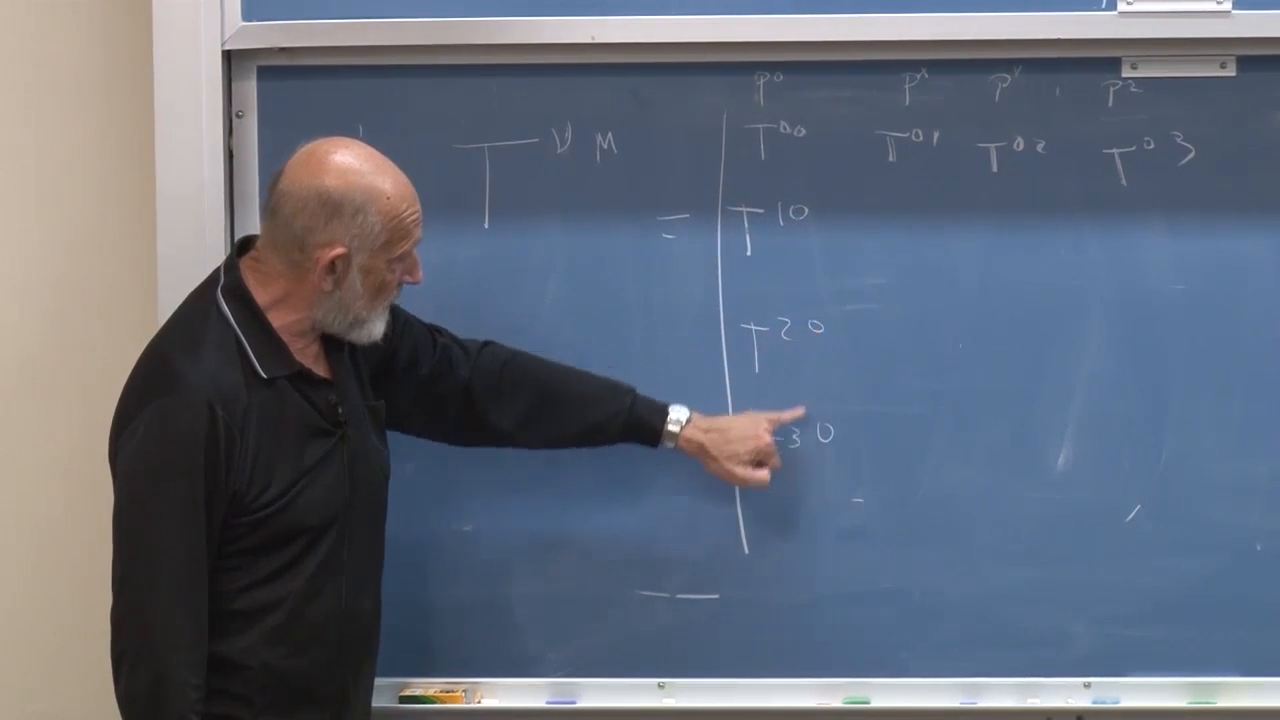
\includegraphics[width=\linewidth]{lecture_10_figure_28.png}
\caption{黑板开始把密度和通量分量整理成能量--动量张量。}
\par\smallskip
\textit{课堂画面：01:51:10。}
\end{figure}

对于所讨论的相对论系统，物理能量--动量张量可以选为对称的：
\begin{equation}
T^{\mu\nu}=T^{\nu\mu}.
\label{eq:stress-energy-symmetry}
\end{equation}
因此，
\begin{equation}
T^{0i}=T^{i0}.
\label{eq:momentum-density-energy-flux}
\end{equation}
当\(c=1\)时，\(i\)动量的密度等于沿\(i\)方向的能量通量。这就是对最后一位听众记忆的回答：坡印廷矢量确实是一种功率密度。

\begin{classroomqa}
\audiencequestion{\(\mathbf E\times\mathbf B\)是功率密度，而不是动量密度吗？}
\lecturerresponse{两者都是。\(T^{\mu\nu}\)的对称性将动量密度\(T^{0i}\)与能量通量\(T^{i0}\)等同起来。因此，\(\mathbf S=\mathbf E\times\mathbf B\)是单位时间单位面积的能量，而在\(c=1\)单位制下，是单位体积的动量。恢复普通单位制后，\(\mathbf g=\mathbf S/c^2\)。
\lecturetimestamp{01:48:20}}
\end{classroomqa}

\begin{figure}[H]
\centering
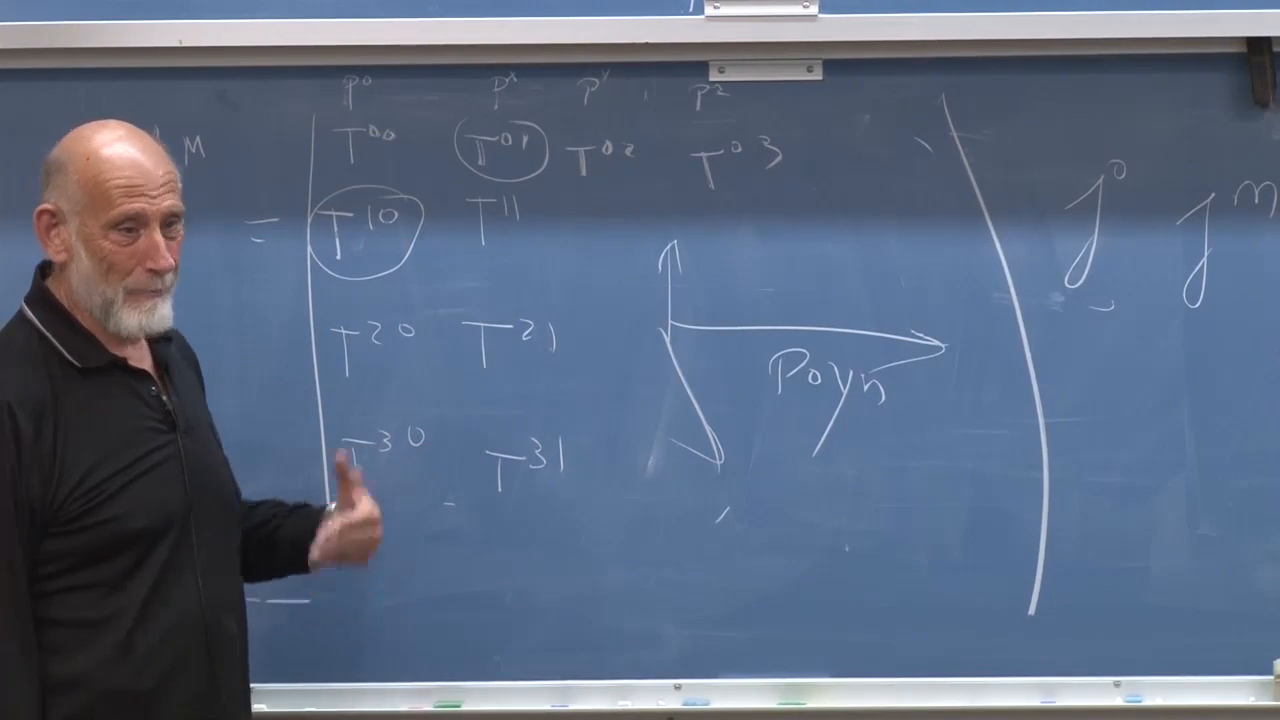
\includegraphics[width=\linewidth]{lecture_10_figure_29.png}
\caption{将动量密度与能量通量等同起来的对称张量关系，在板上以坡印廷矢量标记。}
\par\smallskip
\textit{讲座时间轴：01：53：50。}
\end{figure}

\section{通往广义相对论的桥梁}

本课程以将经典力学、场论和电磁学纳入一个统一结构而告终：
\begin{enumerate}
\item 时间平移不变性给出哈密顿量和能量。
\item 空间平移不变性给出诺特动量。
\item 用空间标记的场取代离散坐标，将求和变为积分，将守恒量变为局域密度。
\item 规范固定揭示出麦克斯韦场的力学坐标，而不改变其可观测量。
\item 麦克斯韦哈密顿量给出
\(\frac12(\mathbf E^2+\mathbf B^2)\)，而空间平移给出
\(\mathbf E\times\mathbf B\)。
\item 对称的能量--动量张量统一了能量密度、动量密度、能量通量和应力。
\end{enumerate}

这正是下一阶段所需的量。在广义相对论中，能量--动量张量作为爱因斯坦场方程中的源出现。因此，最后一讲并非仅仅附加了一个电磁计算；它已经准备好了物质与场告诉时空如何弯曲的语言。
